\documentclass[paper=letterpaper, fontsize=11pt]{scrartcl}
\usepackage[lmargin = 0.75in, rmargin = 0.75in, tmargin = 1in, bmargin = 1in]{geometry}
\usepackage[T1]{fontenc}
\usepackage[english]{babel}
\usepackage{amsmath,amsfonts,amsthm}
\usepackage{sectsty}
\usepackage{fancyhdr}
\usepackage[shortlabels]{enumitem}
\usepackage{xcolor}
\definecolor{tealteal}{rgb}{0.4,0.6,0.6}
\usepackage{hyperref}
\hypersetup{colorlinks = true, allcolors = tealteal}
\usepackage{apacite}
\usepackage{tikz}
\def\checkmark{\tikz\fill[scale=0.4](0,.35) -- (.25,0) -- (1,.7) -- (.25,.15) -- cycle;}
\usepackage{rotating}
\usepackage{placeins}
\usepackage{graphicx}
\usepackage{threeparttable}
\graphicspath{{../figures/}}
\pagestyle{fancyplain}
\fancyhead{}
\fancyfoot[L]{}
\fancyfoot[C]{\thepage}
\fancyfoot[R]{}
\renewcommand{\headrulewidth}{0pt}
\renewcommand{\footrulewidth}{0pt}
\setlength{\headheight}{13.6pt}
\setlength\parindent{0pt}
\newcommand{\horrule}[1]{\rule{\linewidth}{#1}}

\title{	
\normalfont \normalsize 
\textsc{Delaware Valley Regional Planning Commission \\ Southeastern Pennsylvania Pedestrian Counting Program \textit{(19-52-070)}} \\ [25pt]
\huge Technical Reference \\
}
\author{Addison Larson}
\date{\normalsize\today}
\setcounter{section}{-1}

\begin{document}
\renewcommand\UrlFont{\color{tealteal}\rmfamily}
\maketitle

\section{Overview}

\subsection{Purpose}

This paper outlines DVRPC's methodology to select count locations for the Southeastern Pennsylvania Pedestrian Counting Program. The intended outcome of this process is to select count locations that capture the breadth of pedestrian activity in the region. Each location will be counted every three years to monitor changes in pedestrian activity over time.

\subsection{Study area}
The DVRPC Region encompasses nine counties in Pennsylvania and New Jersey. The pedestrian cyclical count program focuses on Bucks, Chester, Delaware, Montgomery, and Philadelphia counties in Pennsylvania. The geographic breadth of the study area and its range of land use and planning contexts---in this case, the City of Philadelphia, suburban, and rural areas---make it difficult to select representative locations for pedestrian counts.

\subsection{Approach}
The site selection process entails four main steps. Sections~\ref{sec:estimate-peds} through~\ref{sec:site-selection} of this paper are dedicated to each of these steps. Section~\ref{sec:estimate-peds} uses publicly available data to estimate average daily pedestrian trips at the census tract level. Section~\ref{sec:test-peds} compares estimated pedestrian densities to observed pedestrian densities using DVRPC's existing pedestrian counts. The results of the comparison are used to test refinements to the pedestrian estimation and modify the estimation formula as necessary. Section~\ref{sec:create-strata} uses the pedestrian estimation and stepwise regressions to create a stratified sampling scheme that divides the region's census tracts into meaningful sampling strata and controls for activity around schools and along road segments with transit service. Section~\ref{sec:site-selection} discusses selecting observations within each sampling stratum and requirements for selecting a count location. The analysis is fully automated in a series of \texttt{R} scripts until Section~\ref{sec:site-selection}, which requires verification of count locations using aerial imagery and site selection in partnership with DVRPC's member governments. \\

DVRPC's member governments provided input throughout the analysis and site selection process. The correspondence between DVRPC and our member governments is documented in Section~\ref{sec:stakeholder-engagement}.\\

Lastly, Section~\ref{sec:improvements} discusses potential methodological improvements.

\subsection{Literature review}
To the best of the authors' knowledge, DVRPC's cyclical pedestrian counting program is the first of its kind in the nation. DVRPC already has an active cyclical bicycle counting program, and the purposes of the bicycle and pedestrian count programs are similar. Both monitor changes in non-motorized activity over time and space by conducting counts at regular intervals for a specified set of locations. However, the site selection process for the bicycle count program only ensured a mixture of facility types (e.g. trail, sidepath, bicycle lane) \cite{dvrpc-bikes}. Given local fluctuations in pedestrian activity, DVRPC sought to take an enhanced approach to selecting count locations in its cyclical pedestrian counting program. \\

The design of DVRPC's pedestrian count program depends on research from North Carolina State University's Institute for Transportation Research and Education (ITRE) \cite{ncstate}, Dr. Sherry Ryan's design of San Diego's non-motorized count program \cite{ryan}, and input from Dr. Krista Nordback at the University of North Carolina Highway Safety Research Center. The ITRE paper was DVRPC's source for the formula for estimating pedestrian trips by census tract and regression analysis to determine the major correlates of pedestrian activity. Dr. Ryan's design of San Diego's non-motorized count program used a 27-strata sampling scheme based on population density, job density, and median household income. DVRPC used Ryan's stratified sampling scheme as a template, substituting the major correlates of pedestrian activity instead of density and income variables to group census tracts into meaningful sampling strata. Dr. Nordback provided invaluable feedback on adequate observations per sampling stratum and on creating additional strata to control for local school and transit activity.

\subsection{Data Sources}
Script \href{https://github.com/addisonlarson/ped_counts/blob/master/1_estimated_peds.R}{\texttt{1\_estimated\_peds.R}} uses the following data sources:
\begin{enumerate}[itemsep=-4pt]
	\item 2017 ACS 5-Year Estimates
	\begin{enumerate}[itemsep=-4pt]
		\item B17004, Poverty status in the past 12 months of individuals by sex by work experience
		\item B08301, Means of transportation to work
		\item B09001, Population under 18 years by age
		\item B14001, School enrollment by level of school for the population 3 years and over
	\end{enumerate}
	\item 2017 National Household Travel Survey (NHTS) Trip File
\end{enumerate}

Script \href{https://github.com/addisonlarson/ped_counts/blob/master/2_observed_peds.R}{\texttt{2\_observed\_peds.R}} uses the following data sources:
\begin{enumerate}[itemsep=-4pt]
	\item 2011-2017 DVRPC Pedestrian Counts
	\item 2017 Circuit Trails Network
\end{enumerate}

Script \href{https://github.com/addisonlarson/ped_counts/blob/master/3_ind_vars.R}{\texttt{3\_ind\_vars.R}} uses the following data sources:
\begin{enumerate}[itemsep=-4pt]
	\item 2017 ACS 5-Year Estimates
	\begin{enumerate}[itemsep=-4pt]
		\item B01003, Total population
		\item B14001, School enrollment by level of school for the population 3 years and over
		\item B17001, Poverty status in the past 12 months of individuals
		\item B08111, Means of transportation to work
		\item B19013, Median household income in the past 12 months
		\item B08014, Sex of workers by vehicles available
		\item B03002, Hispanic or Latino origin by race
	\end{enumerate}
	\item Point locations of libraries, schools serving students in any of the grades K through 8 (public, charter, and magnet) and colleges and universities (incl. public and private)
	\begin{enumerate}[itemsep=-4pt]
		\item Libraries: 2014 OpenStreetMap
		\item Public Schools: 2012-2013 National Center for Education Statistics ELSI Database
		\item Colleges and Universities: 2012-2013 National Center for Education Statistics IPEDS Database
	\end{enumerate}
	\item 2015 LODES Workplace Area Characteristics
	\item Stop-level average weekday transit boards and alights
	\begin{enumerate}[itemsep=-4pt]
		\item Norristown High Speed Line: 2017 SEPTA Automated Passenger Counts (APC) and Ridecheck
		\item Heavy Rail: 2017 SEPTA Turnstile Counts
		\item Bus: 2018 SEPTA APC and Ridecheck
		\item Trolley: 2018 SEPTA APC and Ridecheck
		\item PATCO: 2015 PATCO Turnstile Counts
	\end{enumerate}
	\item 2019 DVRPC Regional Sidewalk Inventory
	\item 2017 PennDOT Crash Statistics
	\item 2017 Philadelphia Litter Index
	\item 2010 DVRPC TransitScore
	\item 2015 DVRPC Land Use
	\item 2016 DVRPC Protected Open Space Inventory
	\item 2017 Pennsylvania DOT Road Centerline
\end{enumerate}

Script \href{https://github.com/addisonlarson/ped_counts/blob/master/5_create_strata.R}{\texttt{5\_create\_strata.R}} uses the following data sources:
\begin{enumerate}[itemsep=-4pt]
	\item Stop-level average weekday transit boards and alights
	\item Point locations of schools serving students in any of the grades K through 8 (public, charter, and magnet)
	\item 2019 Pennsylvania DOT Functional Classification
	\item 2019 City of Philadelphia Functional Classification
\end{enumerate}

\section{Estimate average daily pedestrian trips at the census tract level}
\label{sec:estimate-peds}
Script \href{https://github.com/addisonlarson/ped_counts/blob/master/1_estimated_peds.R}{\texttt{1\_estimated\_peds.R}} estimates the number of daily pedestrian trips at the census tract level. Pedestrian trips are estimated in two phases. First, ACS and NHTS data are used to estimate the sum of pedestrian commute trips for four population groups: employed adults, schoolchildren, college students, and people who work from home. Second, pedestrian commute trips are rescaled to total pedestrian trips using NHTS information on the share of commute trips among all pedestrian trips. \\

Data processing adheres closely to the methodology outlined in the ITRE paper, Appendix B \cite{ncstate}. The main exception is work-from-home pedestrian trips: this paper estimates half the work-from-home pedestrian commute trips of the ITRE paper. See Table~\ref{EstimationMethods} for the input data and calculations used to estimate pedestrian trips and Figure~\ref{estdens} for a map of pedestrian trips standardized by census tract land area.

\begin{table}[!htbp]
	\renewcommand*{\arraystretch}{1.4}
	\caption{Components, calculations, and source data to estimate tract-level daily pedestrian commute trips.}
	\label{EstimationMethods}
	\centering
	\begin{tabular}{|c l c c|} 
		\hline
		\textbf{Component} & \textbf{Description} & \textbf{Source} & \textbf{Calculation} \\
		\hline
		\multicolumn{4}{c}{\textit{Employed adults aged 16 years and older}}\\
		\hline
		a & Total employed persons & B17004 & \\ 
		\hline
		b & Pedestrian commuters & B08301 & \\ 
		\hline
		c & Pedestrian commute percentage & & $\frac{b}{a}$ \\ 
		\hline
		d & Work-at-home & B08301 & \\ 
		\hline
		e & Work-at-home pedestrian commuters & & $\frac{d}{4}$ \\
		\hline
		\multicolumn{4}{c}{\textit{Schoolchildren}}\\
		\hline
		f & Population ages 5-14 & B09001 & \\
		\hline
		g & Estimated school pedestrian share & NHTS & \\
		\hline
		h & School pedestrian commuters & & $f \cdot g$ \\
		\hline
		\multicolumn{4}{c}{\textit{College students}}\\
		\hline
		i & Full-time college students & B14001 & \\
		\hline
		j & College pedestrian commuters & & $i \cdot c$ \\
		\hline
		\multicolumn{4}{c}{\textit{Work and school commute trips subtotal}}\\
		\hline
		k & Daily commuters subtotal & & $ b + e + h + j $ \\
		\hline
		l & Daily commute trips subtotal & & $k \cdot 2$ \\
		\hline
		m & Yearly commute trips subtotal & & $l \cdot 260$ \\
		\hline
		n & Percentage of commute trips in all trips & NHTS & \\
		\hline
		o & Total yearly pedestrian trips & & $\frac{m}{n}$ \\
		\hline
		p & Average daily pedestrian trips & & $\frac{o}{365}$ \\
		\hline
	\end{tabular}
\end{table} 

\begin{figure}[p]
	\centering
	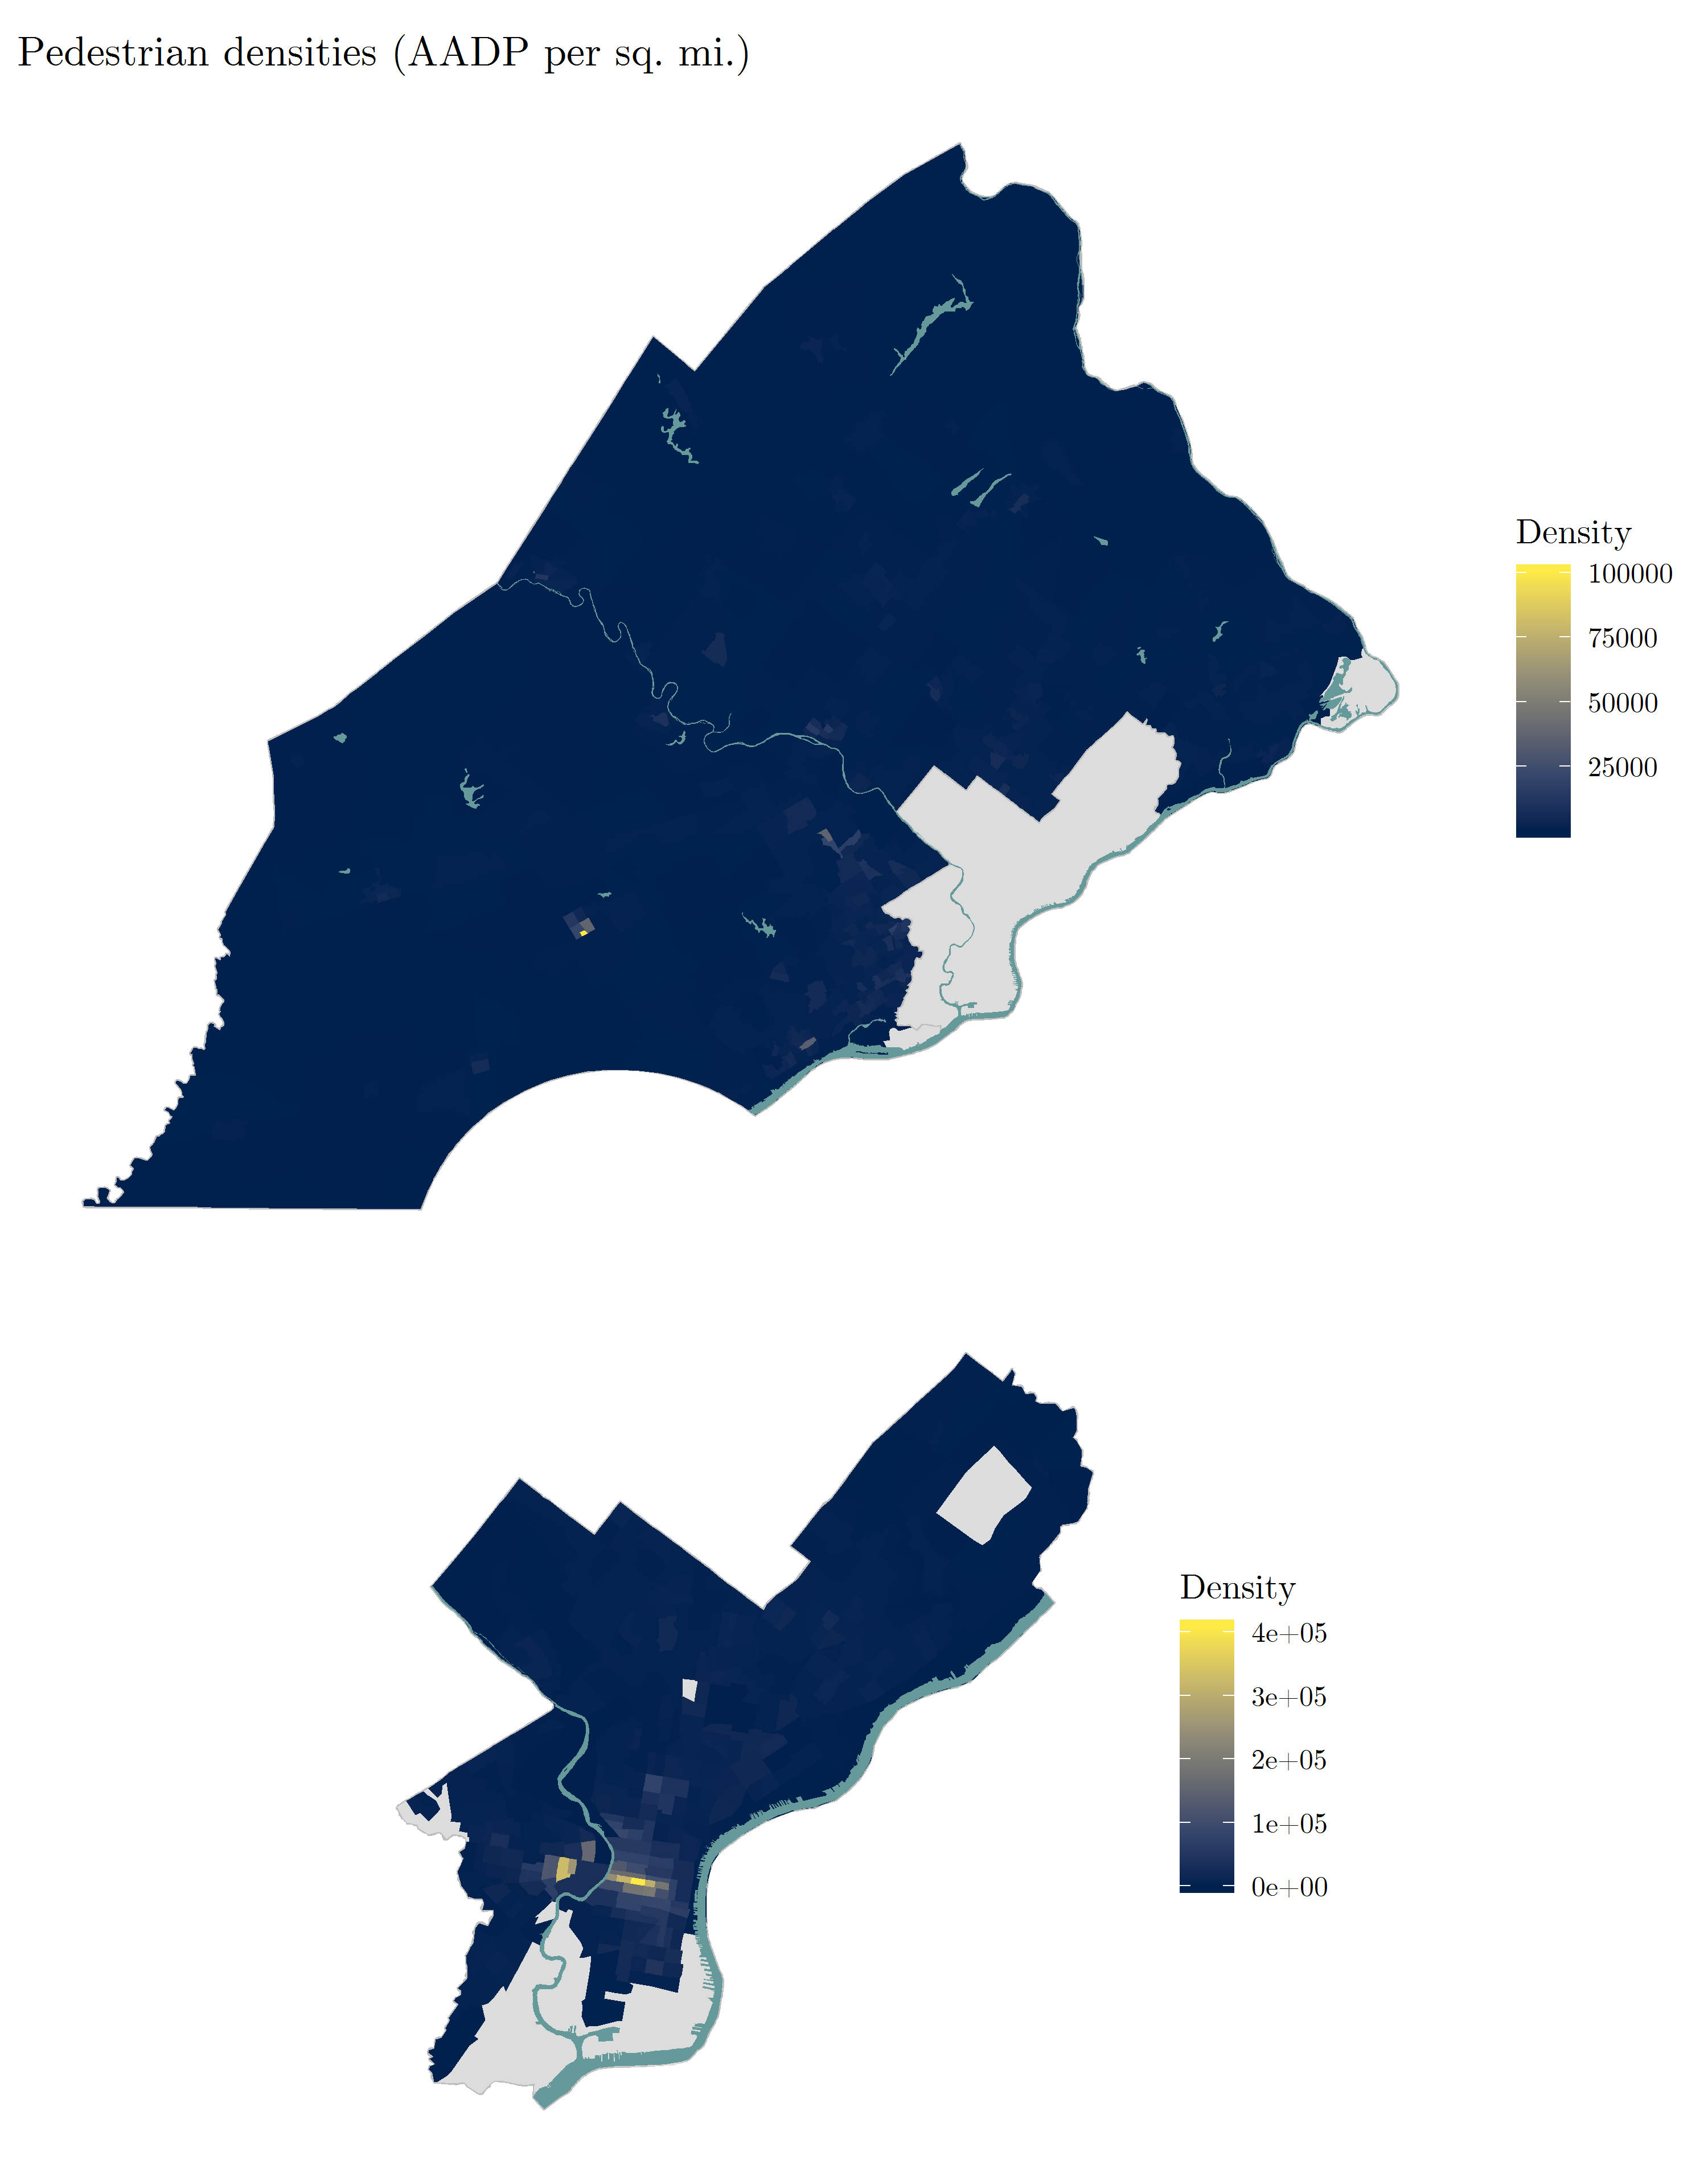
\includegraphics[width = \textwidth]{estdens.png}
	\caption{Estimated pedestrian densities by census tract.} \label{estdens}
\end{figure}

\section{Test and refine pedestrian estimation}
\label{sec:test-peds}
Average daily pedestrian trips at the census tract level are estimated following the ITRE paper's methodology \cite{ncstate}. This section reviews tests of the quality of this pedestrian estimation through IDW interpolation to enable direct comparison between existing pedestrian counts and the pedestrian estimation, mapping linear regression residuals to visualize the contexts where estimated and existing pedestrian trips converge and diverge, and correlation analysis to test the effectiveness of refinements to the pedestrian estimation.

\subsection{IDW interpolation}
DVRPC has conducted 1,127 pedestrian counts in 549 unique locations from 2011 to 2018. However, point-level pedestrian counts are not immediately comparable to census tract-level pedestrian estimates. IDW interpolation and zonal statistics operations transform DVRPC's point-level pedestrian counts to census-tract level pedestrian densities $\left(\frac{AADP}{sq.\:mi.}\right)$, enabling direct comparison between DVRPC's existing counts and the pedestrian estimations computed in Section~\ref{sec:estimate-peds}. See Script \href{https://github.com/addisonlarson/ped_counts/blob/master/2_observed_peds.R}{\texttt{2\_observed\_peds.R}}. \\

IDW creates a continuous raster surface encompassing the maximum extent of existing pedestrian counters. See Figure~\ref{raster-idw} for the IDW output. Each cell in the IDW raster represents the number of expected pedestrians if a count were conducted in that cell. The value of each cell in the raster is imputed from the values of all existing counts in the study area: cells where a pedestrian count has occurred receive the value of this count, and existing counts closer to a given cell receive more influence than counts farther away from that cell. The IDW raster of pedestrians per cell is then overlaid with rasterized census tracts at the same spatial extent and resolution. Finally, a mean pedestrian density per census tract $\left(\frac{AADP}{sq.\:mi.}\right)$ is calculated using the zonal mean. \\

To avoid skewing results, counts within 100 meters of a trail or counts with comments indicating a special or anomalous event are removed from analysis. Locations with multiple counts are assigned the mean of all counts at that location. Leave-one-out cross-validation (LOOCV) is used to select an optimal inverse distance weighting power of 1.5. \\

IDW interpolation is used to \textit{test} the estimations of pedestrians calculated in Section~\ref{sec:estimate-peds}. It cannot \textit{substitute} for the tract-level pedestrian estimations for at least three reasons. First, the physical extent of DVRPC's pedestrian counters is smaller than the study area. This is evident in Figure~\ref{region-count-locations}; the maximum \textit{x}- and \textit{y}-extent of the pedestrian counters does not cover much of Chester and Bucks counties. Substituting the IDW raster for pedestrian estimations would require extrapolating outside the extent of the existing pedestrian counts to cover the entire study area. \\

Second, the spatial coverage of existing pedestrian counts is uneven. See Figures~\ref{phila-count-locations} and \ref{region-count-locations} for maps of pedestrian count locations in the City of Philadelphia and the region, respectively. One of the first visual impressions of Philadelphia's existing count map is a box of closely-spaced counts around Center City Philadelphia; this is DVRPC's cordon line. While IDW cells in Center City Philadelphia rely on the actual values of several nearby counts---from the cordon line, for example---many cells in the suburban counties rely on counts conducted several miles away, in physical contexts possibly quite different. \\

Third, IDW is an exact interpolator, meaning that cells that contain an existing count must inherit that count's value. This method makes cell values subject to outliers; a singularly high or low count affects the value of that cell and all cells in its vicinity. We attempt to address outliers by excluding counts within 100 meters of a trail and with comments designating special or anomalous events. 

\begin{figure}[!htbp]
	\centering
	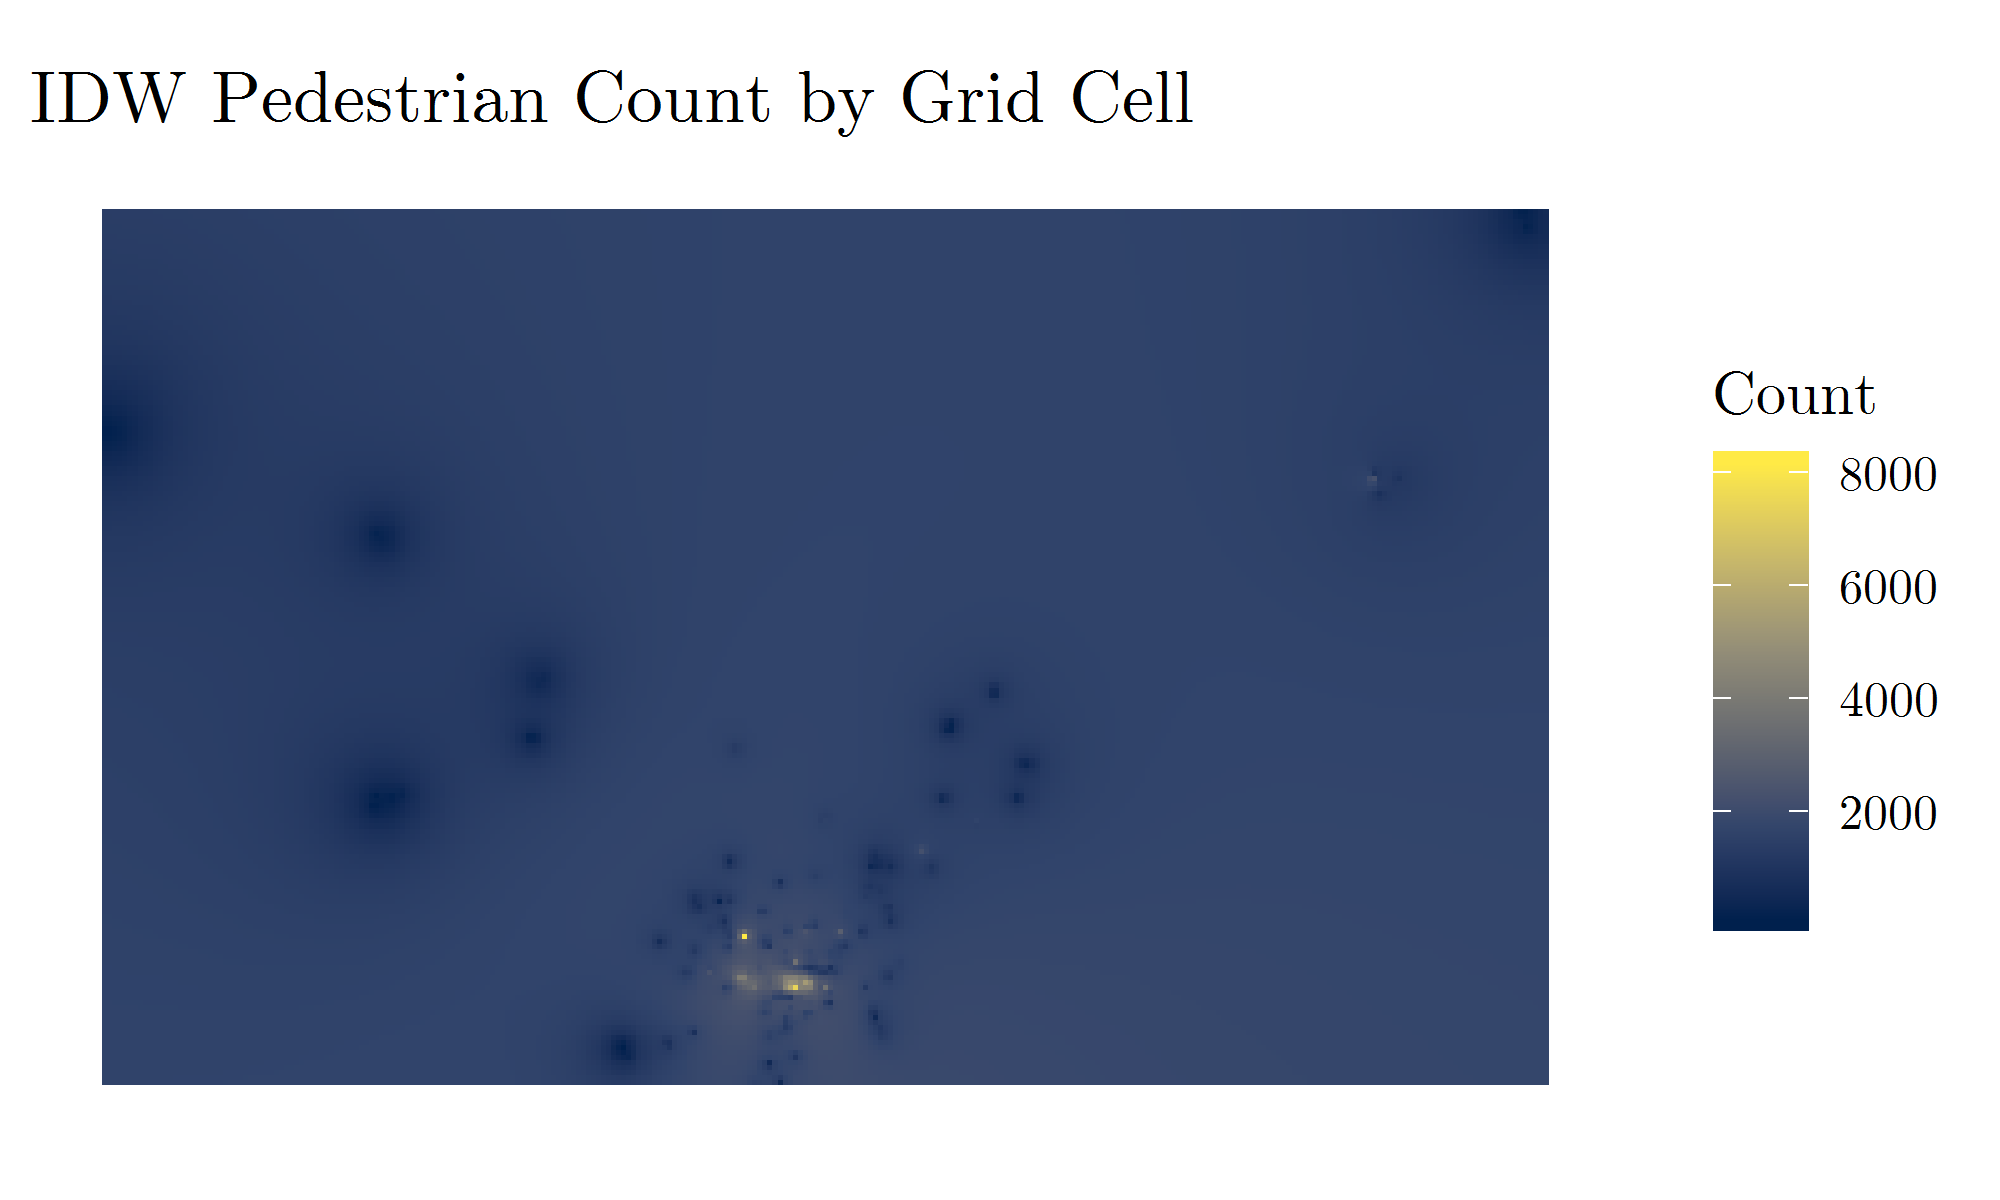
\includegraphics[width = 5in]{idw.png}
	\caption{IDW raster of pedestrian counts. For orientation purposes, the yellow dots are located in Center City Philadelphia. The extent of the IDW raster is smaller than the study area and excludes portions of Chester and Bucks counties.} \label{raster-idw}
\end{figure}

\begin{figure}[!htbp]
	\centering
	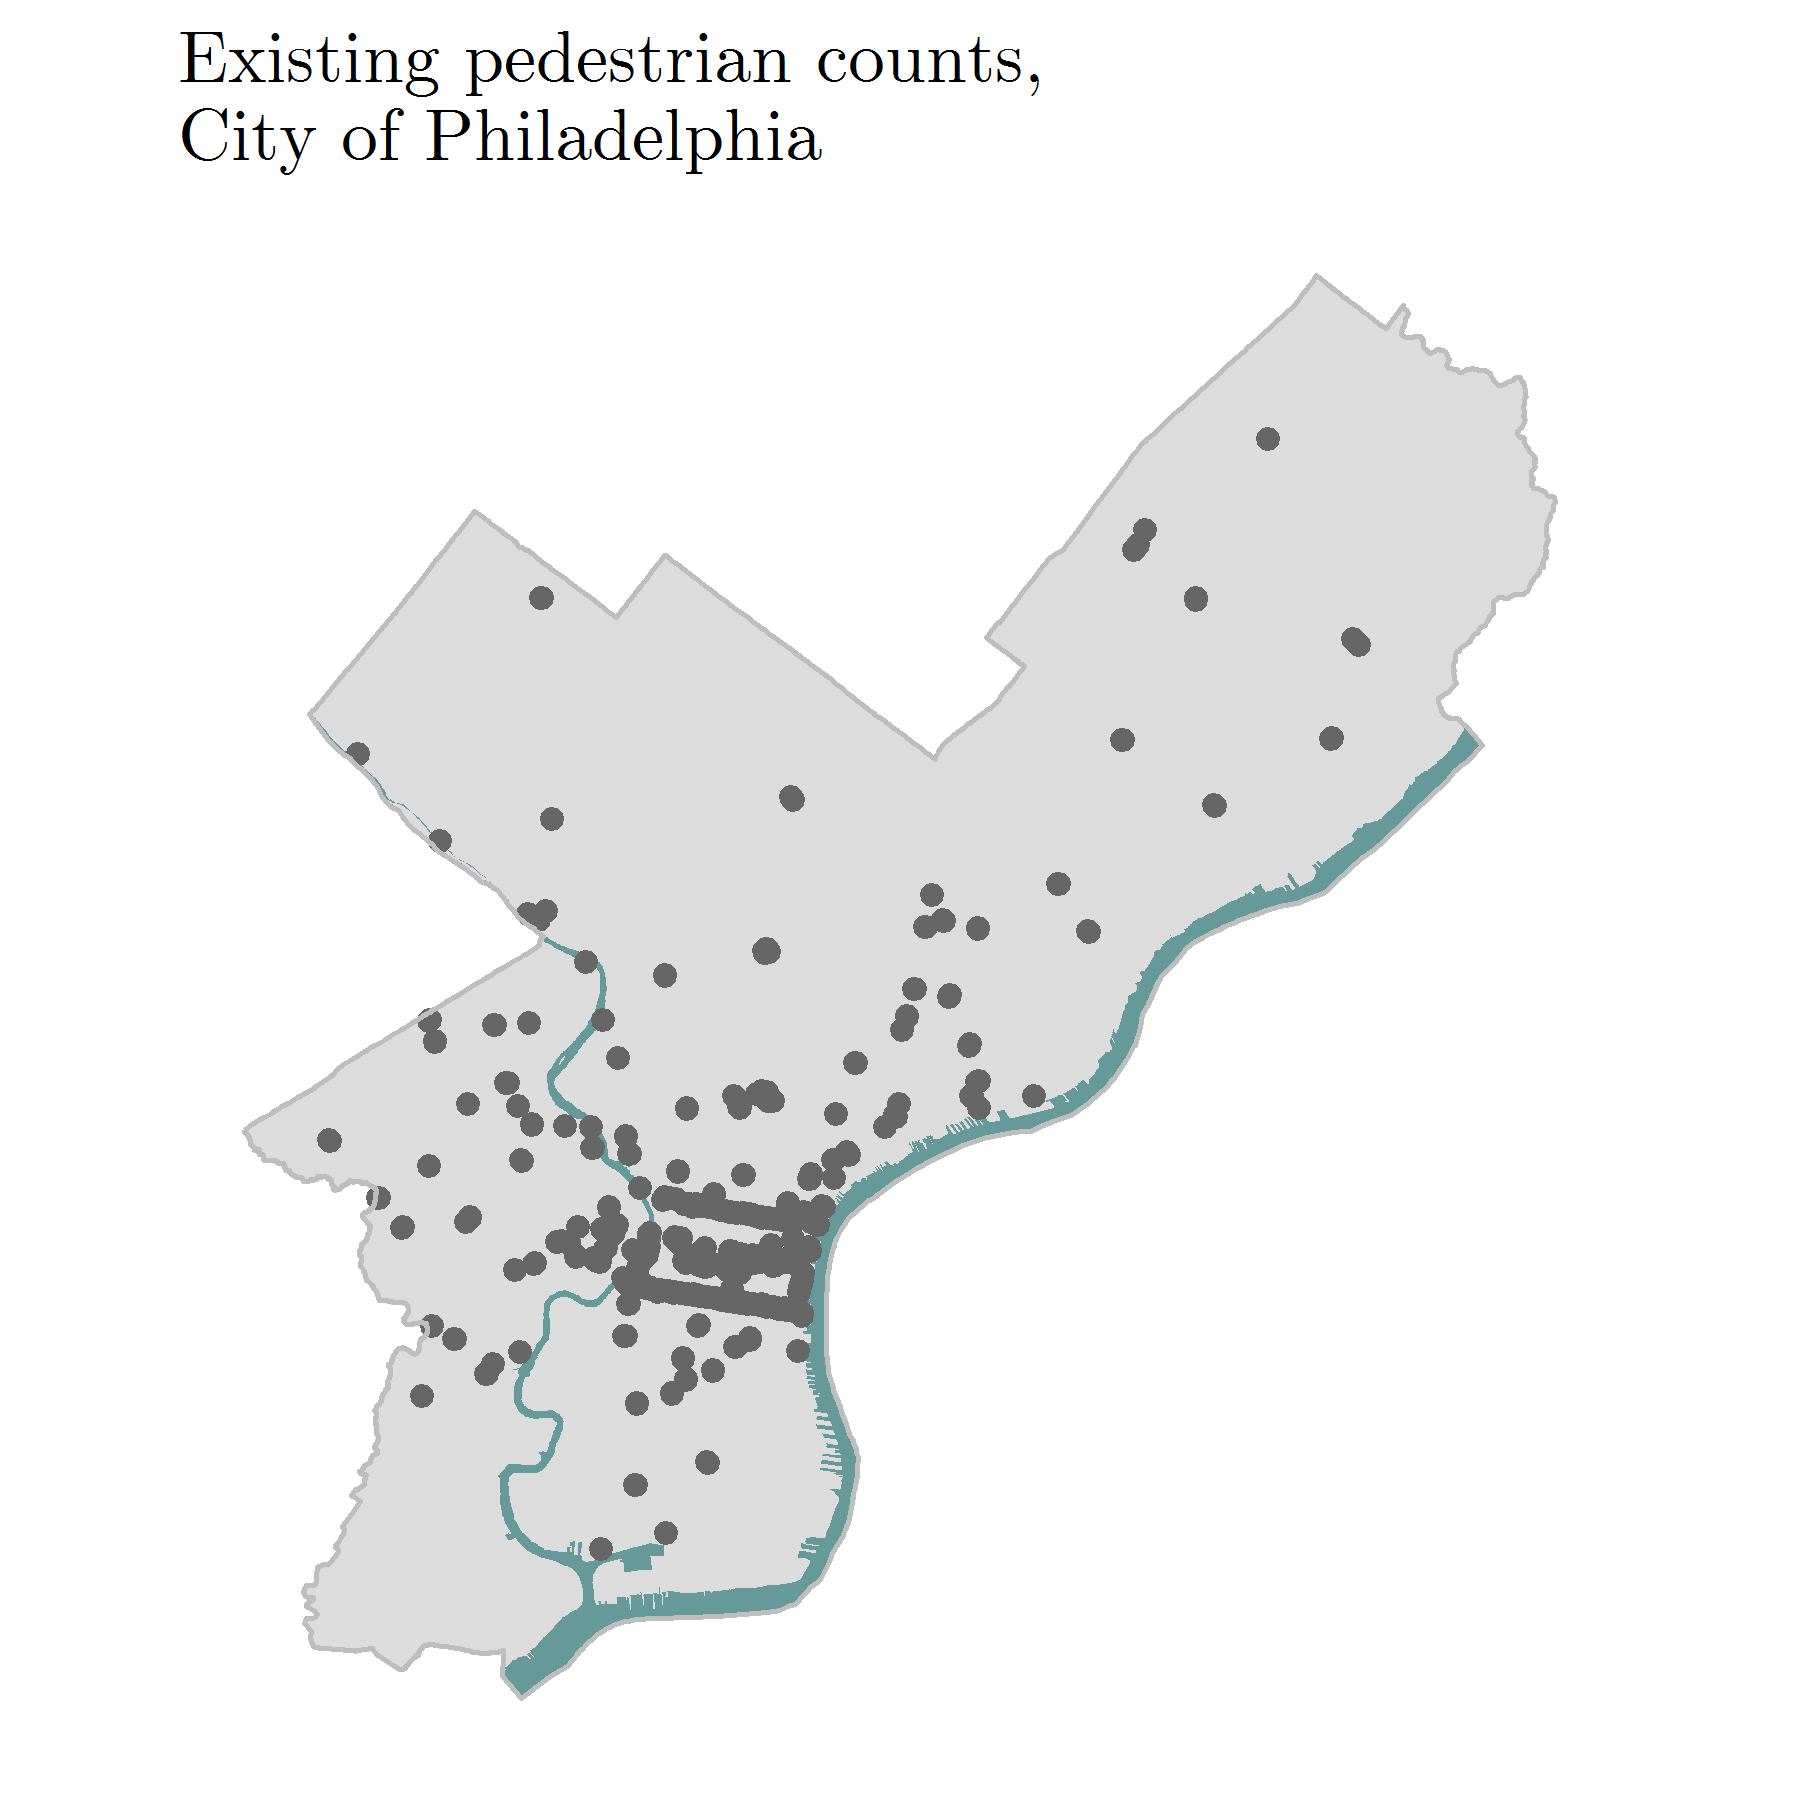
\includegraphics[width = 3.5in]{phila-counters.png}
	\caption{Existing pedestrian count locations in the City of Philadelphia, 2011-2018.} \label{phila-count-locations}
\end{figure}

\FloatBarrier
\begin{sidewaysfigure}[h]
	\centering
	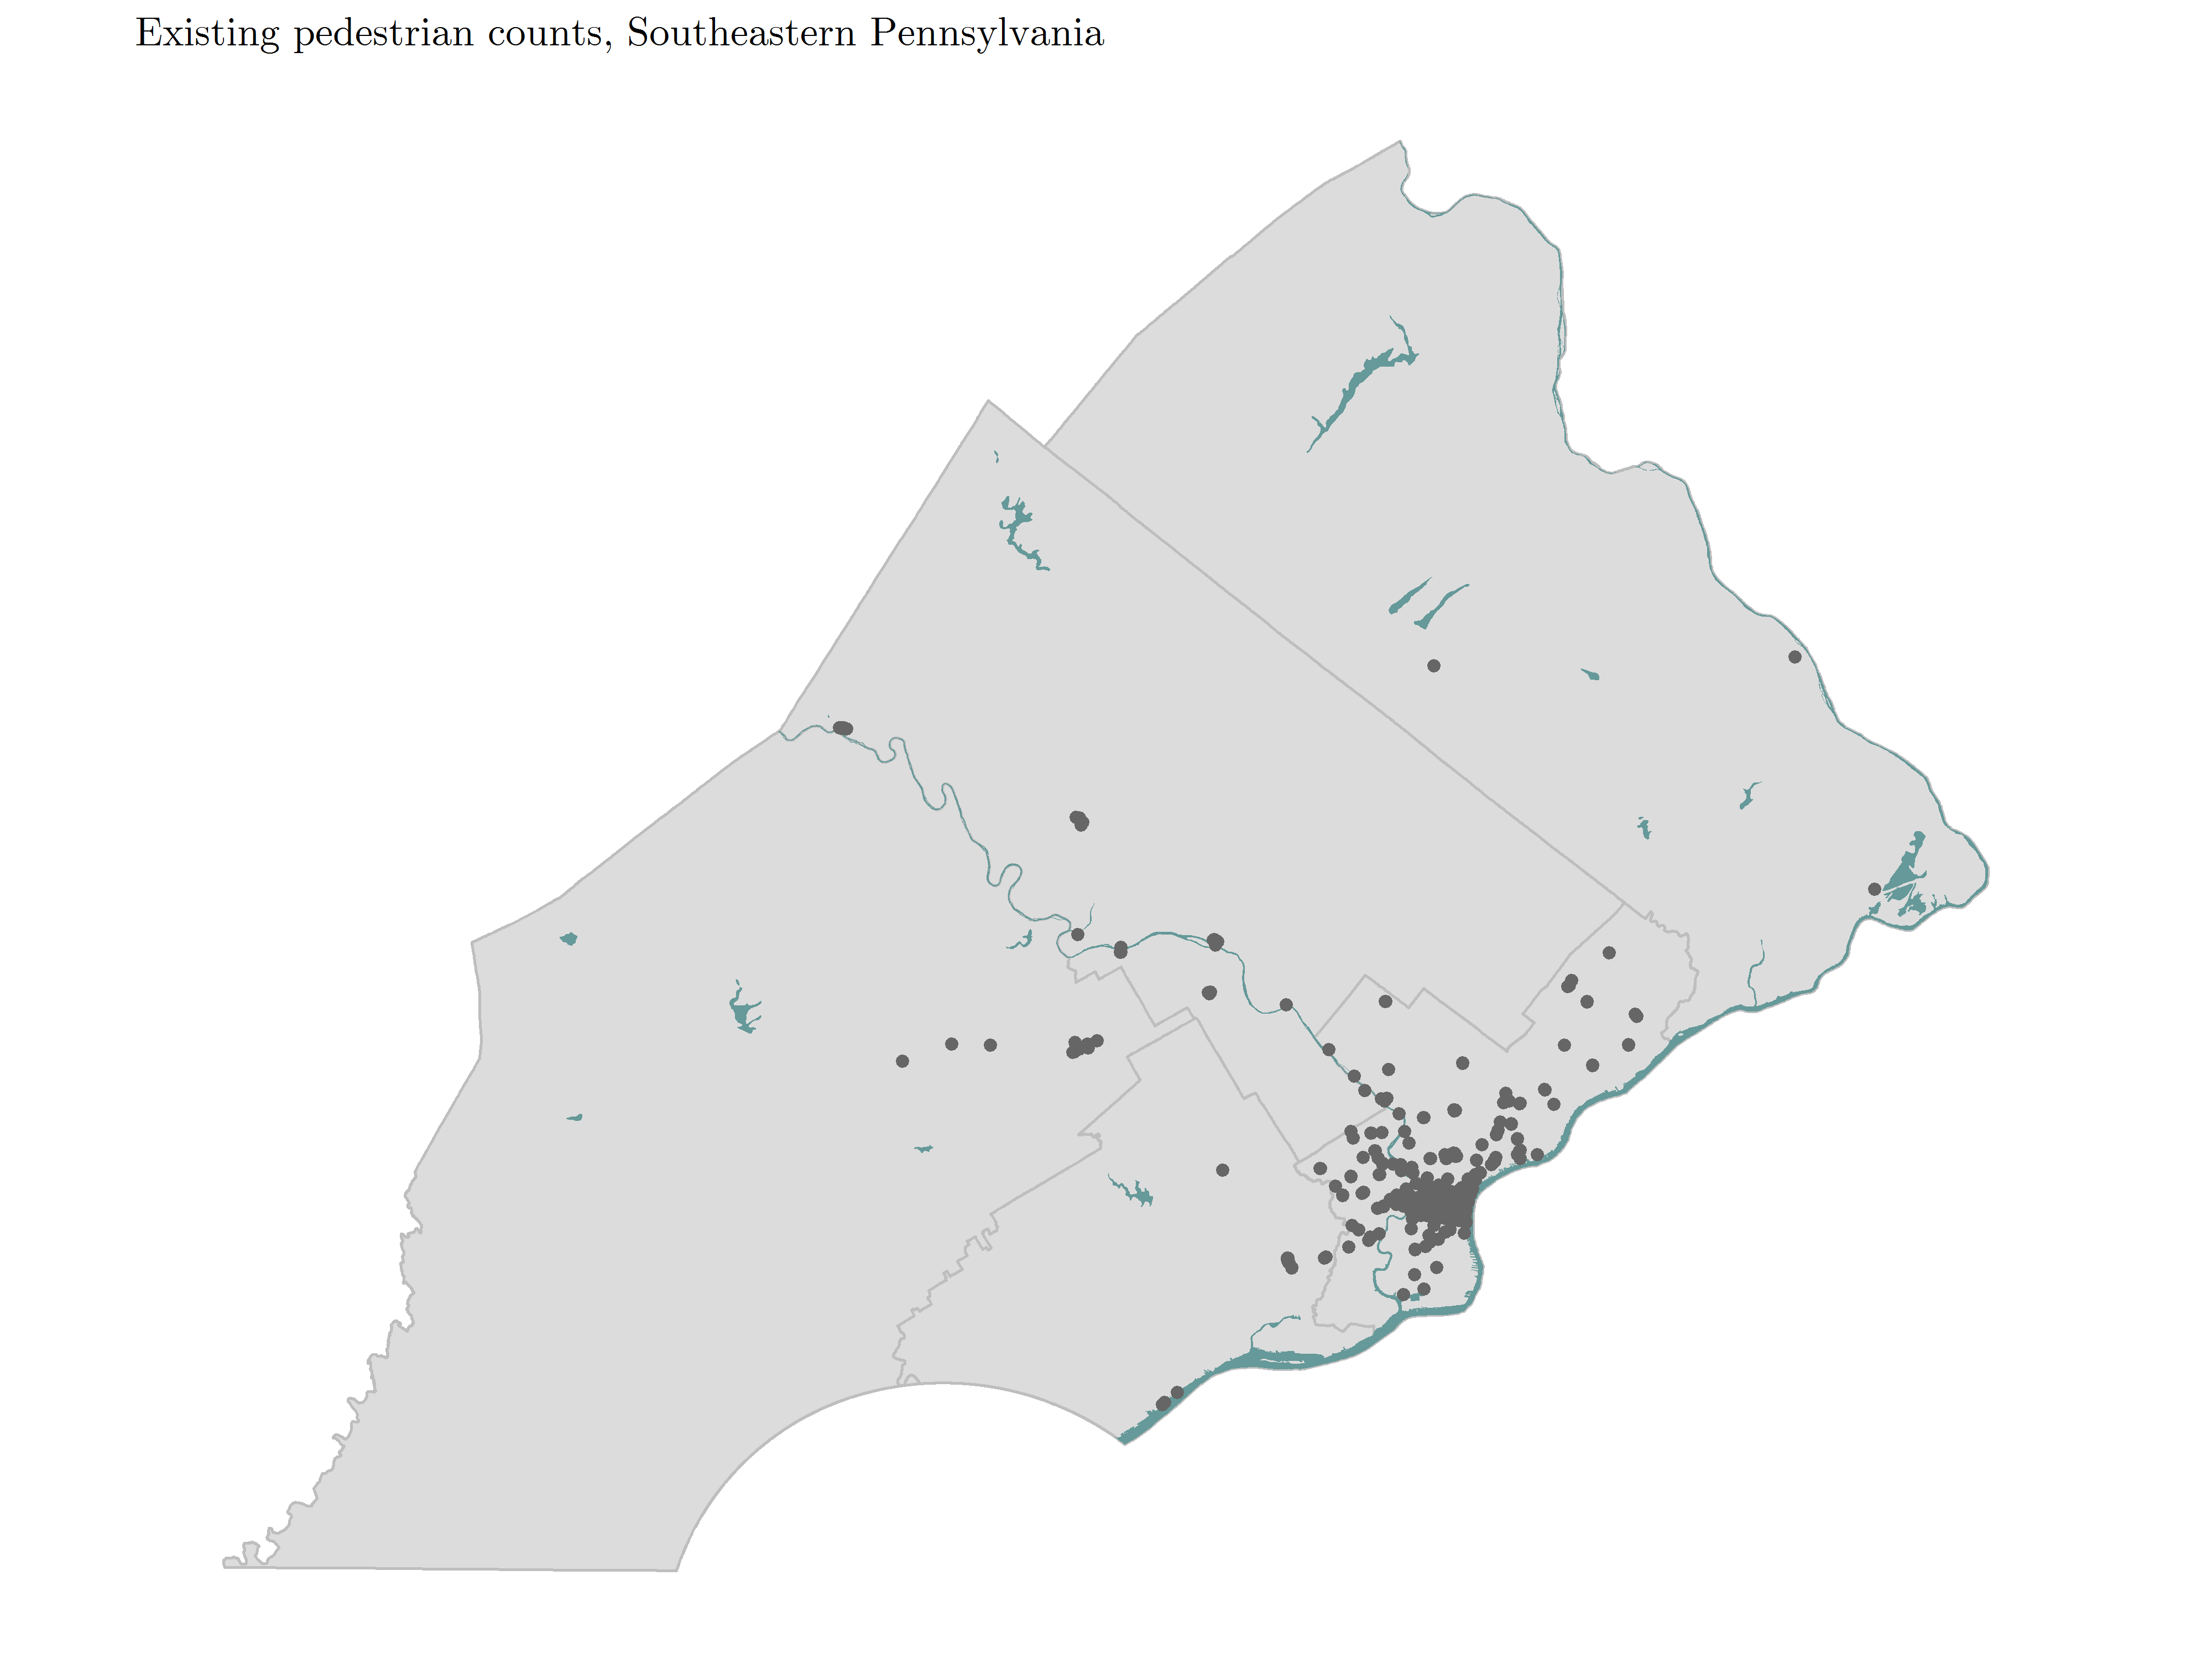
\includegraphics[width = 9in]{region-counters.png}
	\caption{Existing pedestrian count locations in Southeastern Pennsylvania, 2011-2018.} \label{region-count-locations}
\end{sidewaysfigure}
\FloatBarrier

\subsection{Linear regression residuals}

Each census tract has an estimated pedestrian density $\left(\frac{AADP}{sq.\:mi.}\right)$ computed in Section~\ref{sec:estimate-peds} and an actual pedestrian density $\left(\frac{AADP}{sq.\:mi.}\right)$ computed through IDW interpolation. A sinple linear regression model is used to compare the fit of the estimated pedestrian density to the actual pedestrian density. See Table~\ref{r1-fit}. While the model fit is good overall, a map of the regression residuals shown in Figure~\ref{resid} indicates that the pedestrian estimation formula greatly underestimates pedestrian densities in some parts of Center City Philadelphia. The authors suspect the underestimation occurs because the pedestrian estimation does not account for ``last-mile pedestrian commuters,'' those who commute into Center City Philadelphia for school or work.

% Table created by stargazer v.5.2.2 by Marek Hlavac, Harvard University. E-mail: hlavac at fas.harvard.edu
% Date and time: Thu, May 02, 2019 - 10:58:58 AM
\begin{table}[!htbp] \centering 
	\caption{Estimated vs. Observed Pedestrian Density by Tract} 
	\label{r1-fit} 
	\begin{tabular}{@{\extracolsep{5pt}}lc} 
		\\[-1.8ex]\hline 
		\hline \\[-1.8ex] 
		\\[-1.8ex] & Observed Pedestrian Density \\ 
		\hline \\[-1.8ex] 
		Estimated Pedestrian Density & 0.246$^{***}$ \\ 
		& (0.006) \\ 
		& \\ 
		Constant & 2,893.239$^{***}$ \\ 
		& (159.738) \\ 
		& \\ 
		\textit{N} & 861 \\ 
		R$^{2}$ & 0.636 \\ 
		Adjusted R$^{2}$ & 0.636 \\ 
		Residual Std. Error & 4,372.898 (df = 859) \\ 
		F Statistic & 1,503.894$^{***}$ (df = 1; 859) \\ 
		\hline 
		\hline \\[-1.8ex] 
		\textit{Notes:} & \multicolumn{1}{r}{$^{***}$Significant at the 1 percent level.} \\ 
		& \multicolumn{1}{r}{$^{**}$Significant at the 5 percent level.} \\ 
		& \multicolumn{1}{r}{$^{*}$Significant at the 10 percent level.} \\ 
	\end{tabular} 
\end{table} 

\FloatBarrier
\begin{sidewaysfigure}[h]
	\centering
	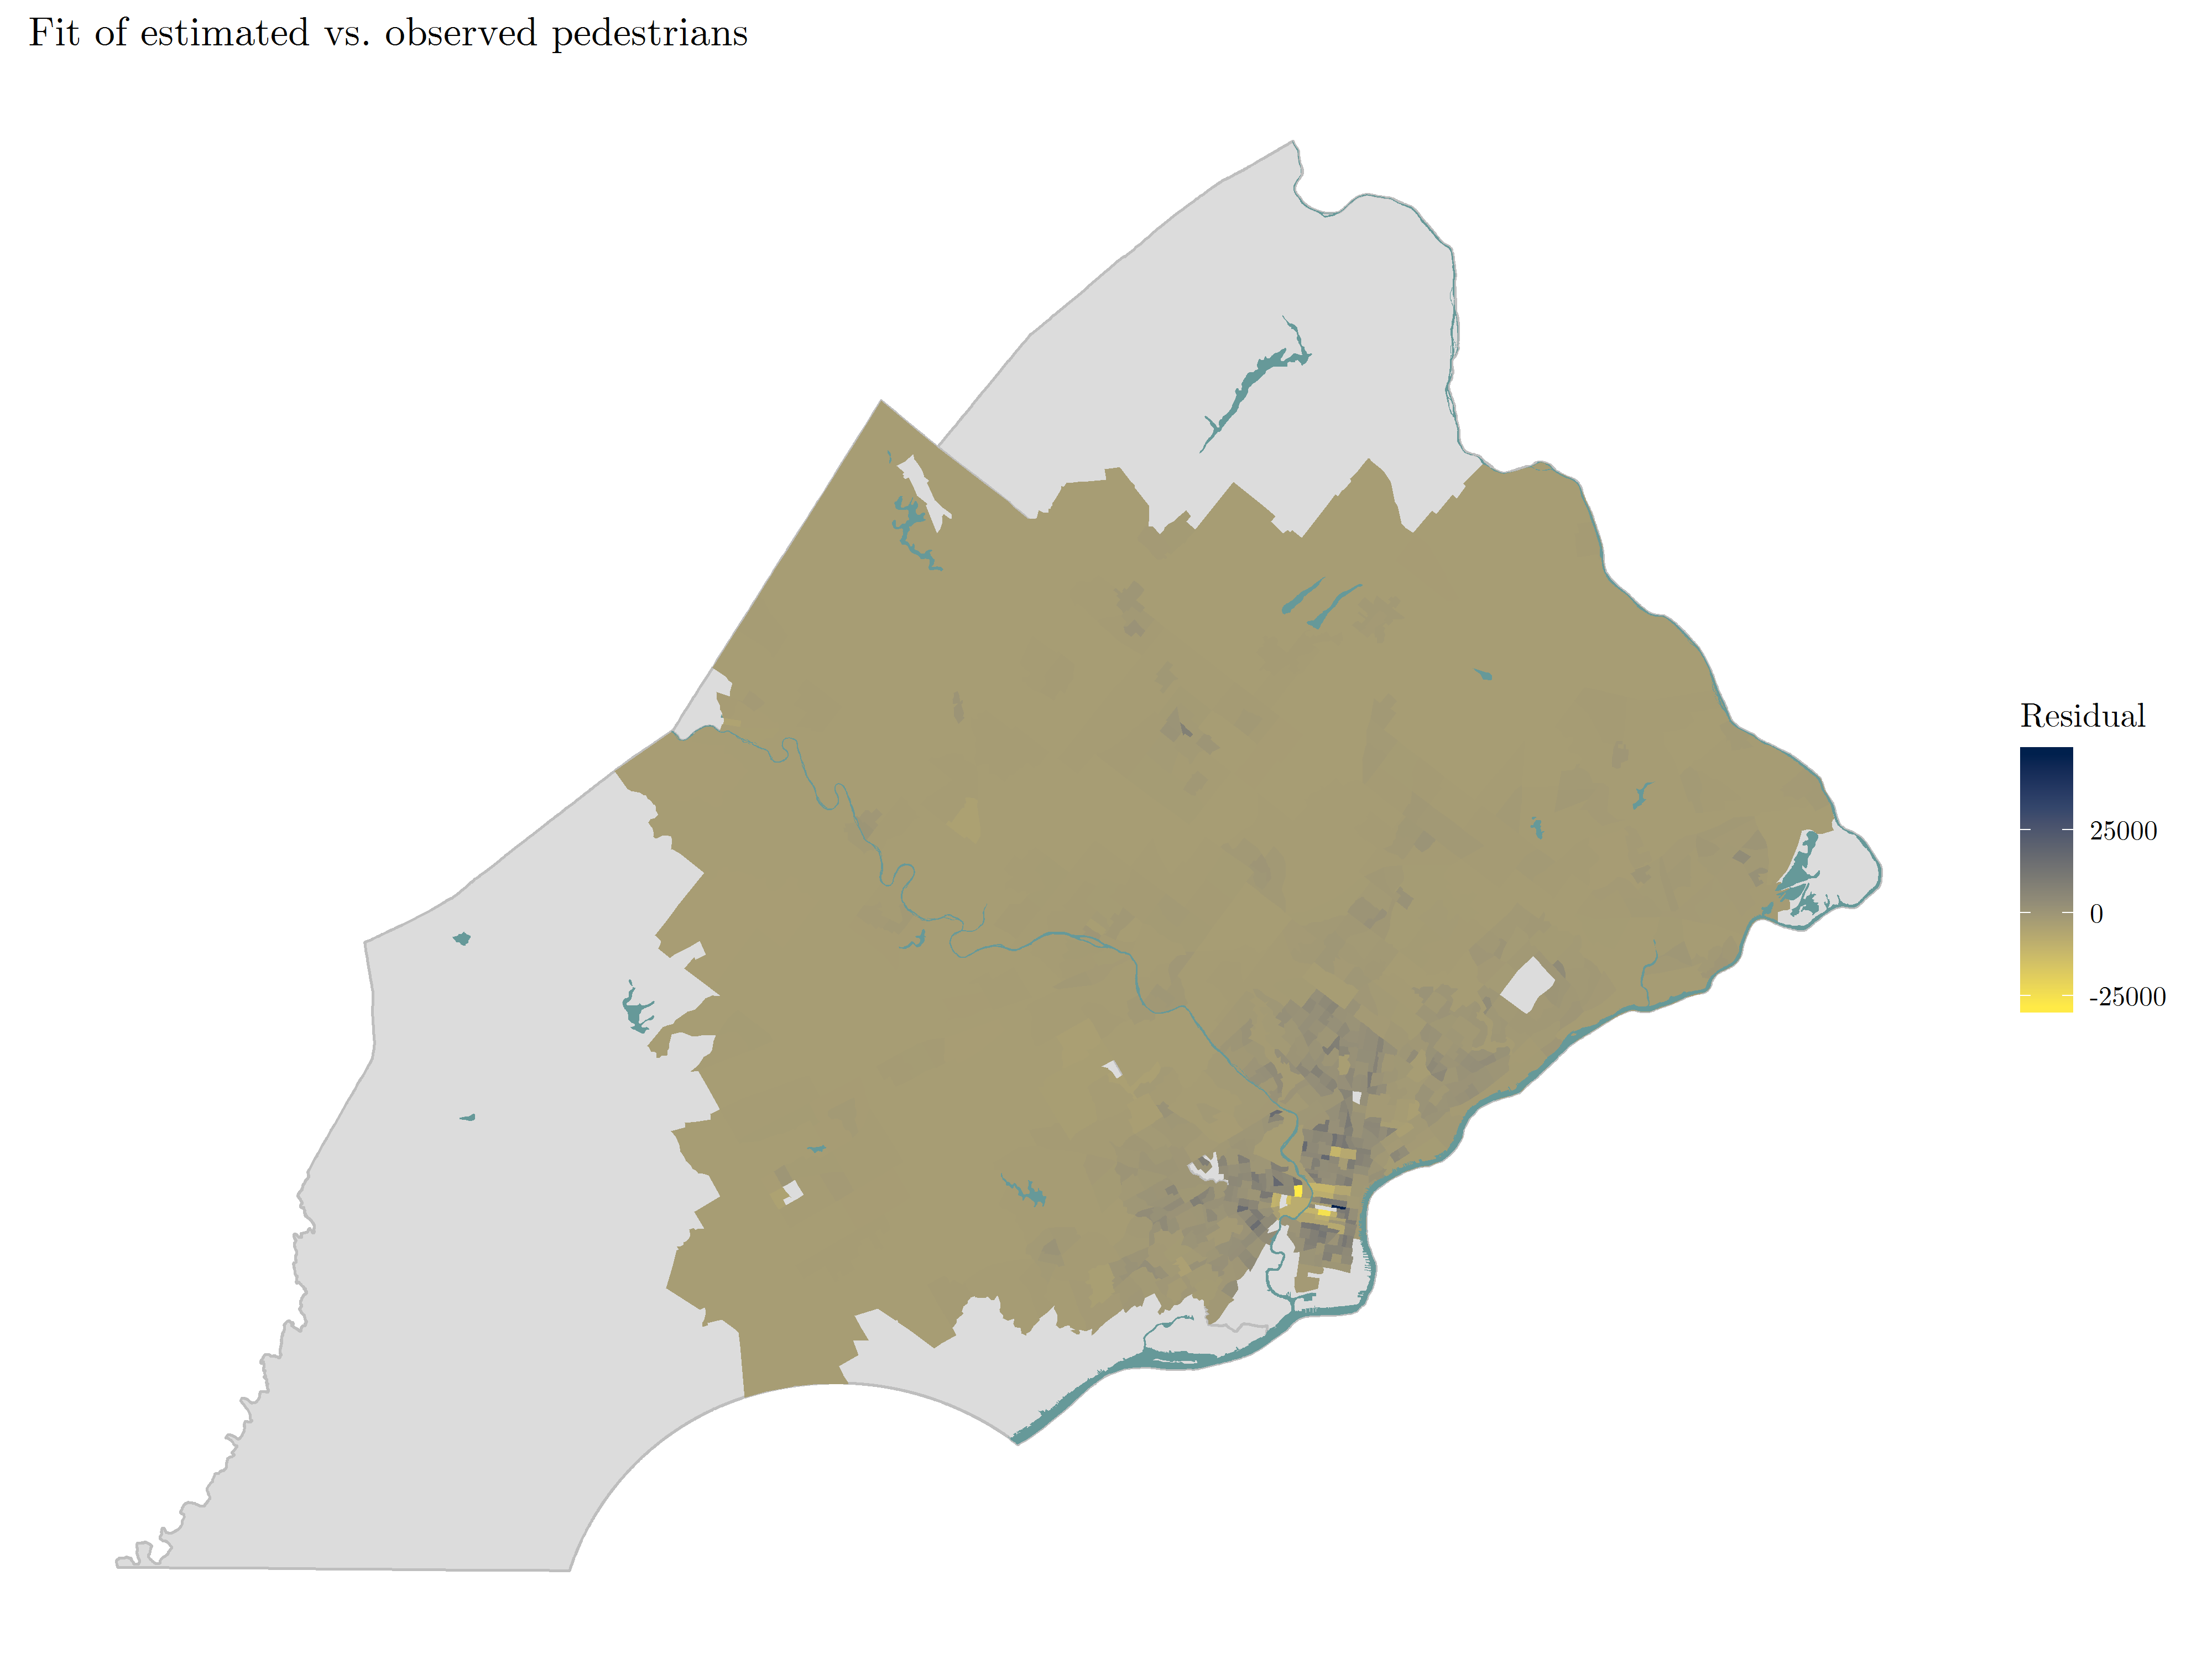
\includegraphics[width = 9in]{resid.png}
	\caption{Assessing fit of estimated vs. observed pedestrian densities $\left(\frac{AADP}{sq.\:mi.}\right)$. One tract in University City, in yellow, has an observed pedestrian density far less than the estimate, perhaps driven by an outlier count. Two census tracts in Center City, in dark blue, have observed pedestrian densities far greater than the estimate.} \label{resid}
\end{sidewaysfigure}
\FloatBarrier

\subsection{Pedestrian estimation refinements and correlation analysis}

Given the underestimations in Center City, ``last-mile pedestrian commuters'' were estimated in five ways, added to the estimated average daily pedestrian trips, and compared to the actual pedestrian density obtained through IDW interpolation. The list below describes each refinement and its correlation with actual pedestrian density.

\begin{itemize}[itemsep=-4pt]
	\item \textit{No change:} implement methodology from the ITRE paper \cite{ncstate}. $r = 0.830$.
	\item \textit{R1:} Percentage transit commuters in the DVRPC Region $\cdot$ Count of Regional Rail stations in tract $\cdot$ Number of jobs in tract.\footnote{For the number of jobs in a census tract, we remove jobs where the origin tract and destination tract are the same. We assume these commuters are already captured in the original pedestrian estimation. This approach applies to all refinements.} $r = 0.769$.
	\item \textit{R2:} Percentage transit commuters in the DVRPC Region $\cdot$ Boolean indicating presence of Regional Rail station in tract $\cdot$ Number of jobs in tract. $ r =0.782$.
	\item \textit{R3:} Station-level Regional Rail alights. $r = 0.429$.
	\item \textit{R4:} Use a proportionality constant between station-level Regional Rail alights and the number of jobs in the tract to infer Regional Rail alights where ridership data is missing. $r = 0.480$.
	\item \textit{R5:} Same as R4, but assume that Regional Rail riders have work destinations not only in tracts containing Regional Rail stations, but also tracts that are rook contiguous with Regional Rail station tracts. $r = 0.592$.
\end{itemize}

The correlation between estimated and actual pedestrian densities is highest for the original pedestrian estimation. Therefore, the original pedestrian estimation is used in regression analysis.

\section{Strata creation}
\label{sec:create-strata}
Three types of sampling strata are created to ensure a representative mix of locations and contexts for pedestrian counting. \\

Census tract sampling strata are comprised of census tracts differentiated by the highest correlates of pedestrian activity. These correlates are selected using stepwise regression among several demographic, land use, and transportation-related attributes of each census tract. Regressions are computed separately for Philadelphia and the suburbs, creating two separate sets of census tract sampling strata. By using regression analysis to inform the creation of our sampling strata, the region's census tracts are grouped in a way that correlates with changes in pedestrian densities. See Script \href{https://github.com/addisonlarson/ped_counts/blob/master/4_regressions.R}{\texttt{4\_regressions.R}}. \\

Transit arterial strata are road segments differentiated by their levels of transit service. It is expected that transit access drives pedestrian activity at a spatial level more granular than the census tract. For example, a pedestrian counter placed along a road segment with a trolley station is expected to have more pedestrian activity than a road segment one block away with no transit service, all else held equal. The transit arterial strata are created separately for Philadelphia and the suburbs, using different input files and definitions of ``transit service.'' \\

The school sampling stratum is created only for the suburban counties. Similar to transit arterials, elementary and middle schools are expected to drive pedestrian activity in the suburbs at a small area level. \\

The transit arterial and school sampling strata are erased from the underlying census tracts. This makes it impossible to select a census tract count location that is near school grounds or a bus stop along a major arterial, for example. See Script \href{https://github.com/addisonlarson/ped_counts/blob/master/5_create_strata.R}{\texttt{5\_create\_strata.R}}.

\subsection{Census tract sampling strata}
Creating a stratified sampling scheme for census tracts requires three steps. First, a series of independent variables at the census tract level are prepared for use in regression analyses. These variables include demographic, land use, and infrastructure characteristics of each census tract. Second, stepwise regressions determine the primary correlates of pedestrian activity, where the dependent variable is the pedestrian estimation computed in Section~\ref{sec:estimate-peds}. Regressions are computed separately for the City of Philadelphia and the region's suburban counties, as these are expected to have different pedestrian patterns. Once the correlates are identified, they are used to group census tracts into sampling strata. Because regressions are run separately for Philadelphia and the suburbs, there are two sets of census tract sampling strata.

\subsubsection{Prepare tract-level independent variables for regression analysis}

Many independent variables require data preparation, areal interpolation, and computing densities. Script \href{https://github.com/addisonlarson/ped_counts/blob/master/3_ind_vars.R}{\texttt{3\_ind\_vars.R}} prepares independent variables. See Table~\ref{IndependentVariables} for details on the independent variables computed, including descriptions and data sources. All variables are computed at the tract level, which sometimes requires aggregating point data or areal interpolation of smaller geographic units, such as blocks or Traffic Analysis Zones (TAZs), to the census tract level. These instances are noted in the \textit{Calculation} column in Table~\ref{IndependentVariables}. Density-based measures use two different land area calculations in the denominator. The first, \textit{waterless}, excludes water from the total census tract area. The second, \textit{unprotected}, excludes both water and protected land uses from the total census tract area. The denominator is noted in the \textit{Source} column in Table~\ref{IndependentVariables}. \\

Five variables were created in this script for use in regressions and removed later for one or more of three principal reasons. First, some variables posed a \textit{multicollinearity risk} in regressions. Second, some variables were determined to have \textit{reduced utility} in creating a stratified sampling scheme because observations were ubiquitous or rare. Third, DVRPC substituted different variables when there was \textit{better data available}. The five variables removed from analysis and their justification for removal are described below.

\begin{enumerate}[itemsep=-4pt]
	\item Urban Boolean $\left(\frac{1,280+\:persons}{sq.\:mi.}\right)$. \textit{Reduced utility}: Most census tracts in the study area qualify as ``urban.'' The mean and median population densities are 9,772 and 5,340 people per square mile; of the 987 census tracts with estimated total population greater than or equal to 100, only 168 (17.02\%) do \textit{not} qualify as ``urban.''
	\item University Boolean (50+\% of tract population are students \textit{or} university is present). \textit{Multicollinearity risk}: This variable correlates almost perfectly with the census tract percentage of college students. \textit{Reduced utility}: Census tracts containing universities are relatively rare in the region. If we aim to understand pedestrian trends specifically around universities, then we can conduct project-specific counts around universities.
	\item School counts (Number of schools serving students in any of the grades K through 8 per census tract). \textit{Reduced utility}: We create a separate sampling stratum for suburban schools, so this variable is not needed in regressions.
	\item Library counts (Number of libraries per census tract). \textit{Reduced utility}: Libraries are rare, and their distribution is highly skewed. Most census tracts have zero libraries, but one tract has nine.
	\item Transit use per capita (Expected transit commute trips extrapolated from ACS Table B08111). \textit{Better  data available}: We substitute this measure with ``transit activity density,'' which relies on stop-level ridership data instead of survey responses based on a commuter's home census tract.
\end{enumerate}

\begin{table}
	\centering
	\begin{threeparttable}
		\renewcommand*{\arraystretch}{1.4}
		\caption{Calculations and source data to compute independent variables.}
		\label{IndependentVariables}
		\centering
		\begin{tabular}{|p{\dimexpr 0.4\linewidth-2\tabcolsep} p{\dimexpr 0.3\linewidth-2\tabcolsep} p{\dimexpr 0.3\linewidth-2\tabcolsep} |} 
			\hline
			\textbf{Variable} & \textbf{Calculation} & \textbf{Source} \\
			\hline
			Population density & $\left(\frac{persons\:(1000s)}{sq.\:mi.}\right)$ & B01003, \textit{unprotected} \\ 
			\hline
			Pct. of population enrolled in college & & B14001 \\ 
			\hline
			Job density & $\left(\frac{jobs\:(1000s)}{sq.\:mi.}\right)$ & LODES, \textit{unprotected} \\
			\hline
			Pct. of households below FPL & & B17001 \\
			\hline
			Transit activity density & $\left(\frac{transit\:boards\:+\:alights}{sq.\:mi.}\right)$ & Ridership, \textit{unprotected} \\
			\hline
			Sidewalk density & $\left(\frac{length\:(mi.)}{sq.\:mi.}\right)$ & Sidewalk network, \textit{waterless} \\
			\hline
			Median household income, \$1000s & & B19013 \\
			\hline
			Pct. of zero-car households & & B08014 \\
			\hline
			Pct. of nonwhite residents & & B03002 \\
			\hline
			No. of pedestrian crashes in tract & Point aggregated to tract & PennDOT Crash Statistics \\
			\hline
			Philadelphia Litter Index & Block interpolated to tract & \\
			\hline
			DVRPC TransitScore & TAZ interpolated to tract & \\
			\hline
			Land use mix & $\left(\frac{Herfindahl-Hirschman\:Index}{100}\right)$ & DVRPC Land Use \\
			\hline
			Pct. of pedestrian commuters & & B08111 \\
			\hline
			Sidewalk-to-road ratio \tnote{2} & $\left(\frac{sidewalk\:length}{road\:centerline\:length}\right)$ & Sidewalk network, PA Centerline\\
			\hline
			Road density & $\left(\frac{length\:(mi.)}{sq.\:mi.}\right)$ & \textit{waterless} \\
			\hline
			People density & $\left(pop.\:dens.+job\:dens. \right)$ & B01003, LODES \\
			\hline
			People interaction effect & $\left(pop.\:dens.\cdot job\:dens.\right)$ & B01003, LODES \\
			\hline
		\end{tabular}
		\begin{tablenotes}
			\item[2] A sidewalk-to-road ratio of 2 indicates full sidewalk coverage on both sides of every road. Limited access roads are removed from the centerline shapefile before processing. See Figure~\ref{srr}.
		\end{tablenotes}
	\end{threeparttable}
\end{table}

\FloatBarrier
\begin{sidewaysfigure}[h]
	\centering
	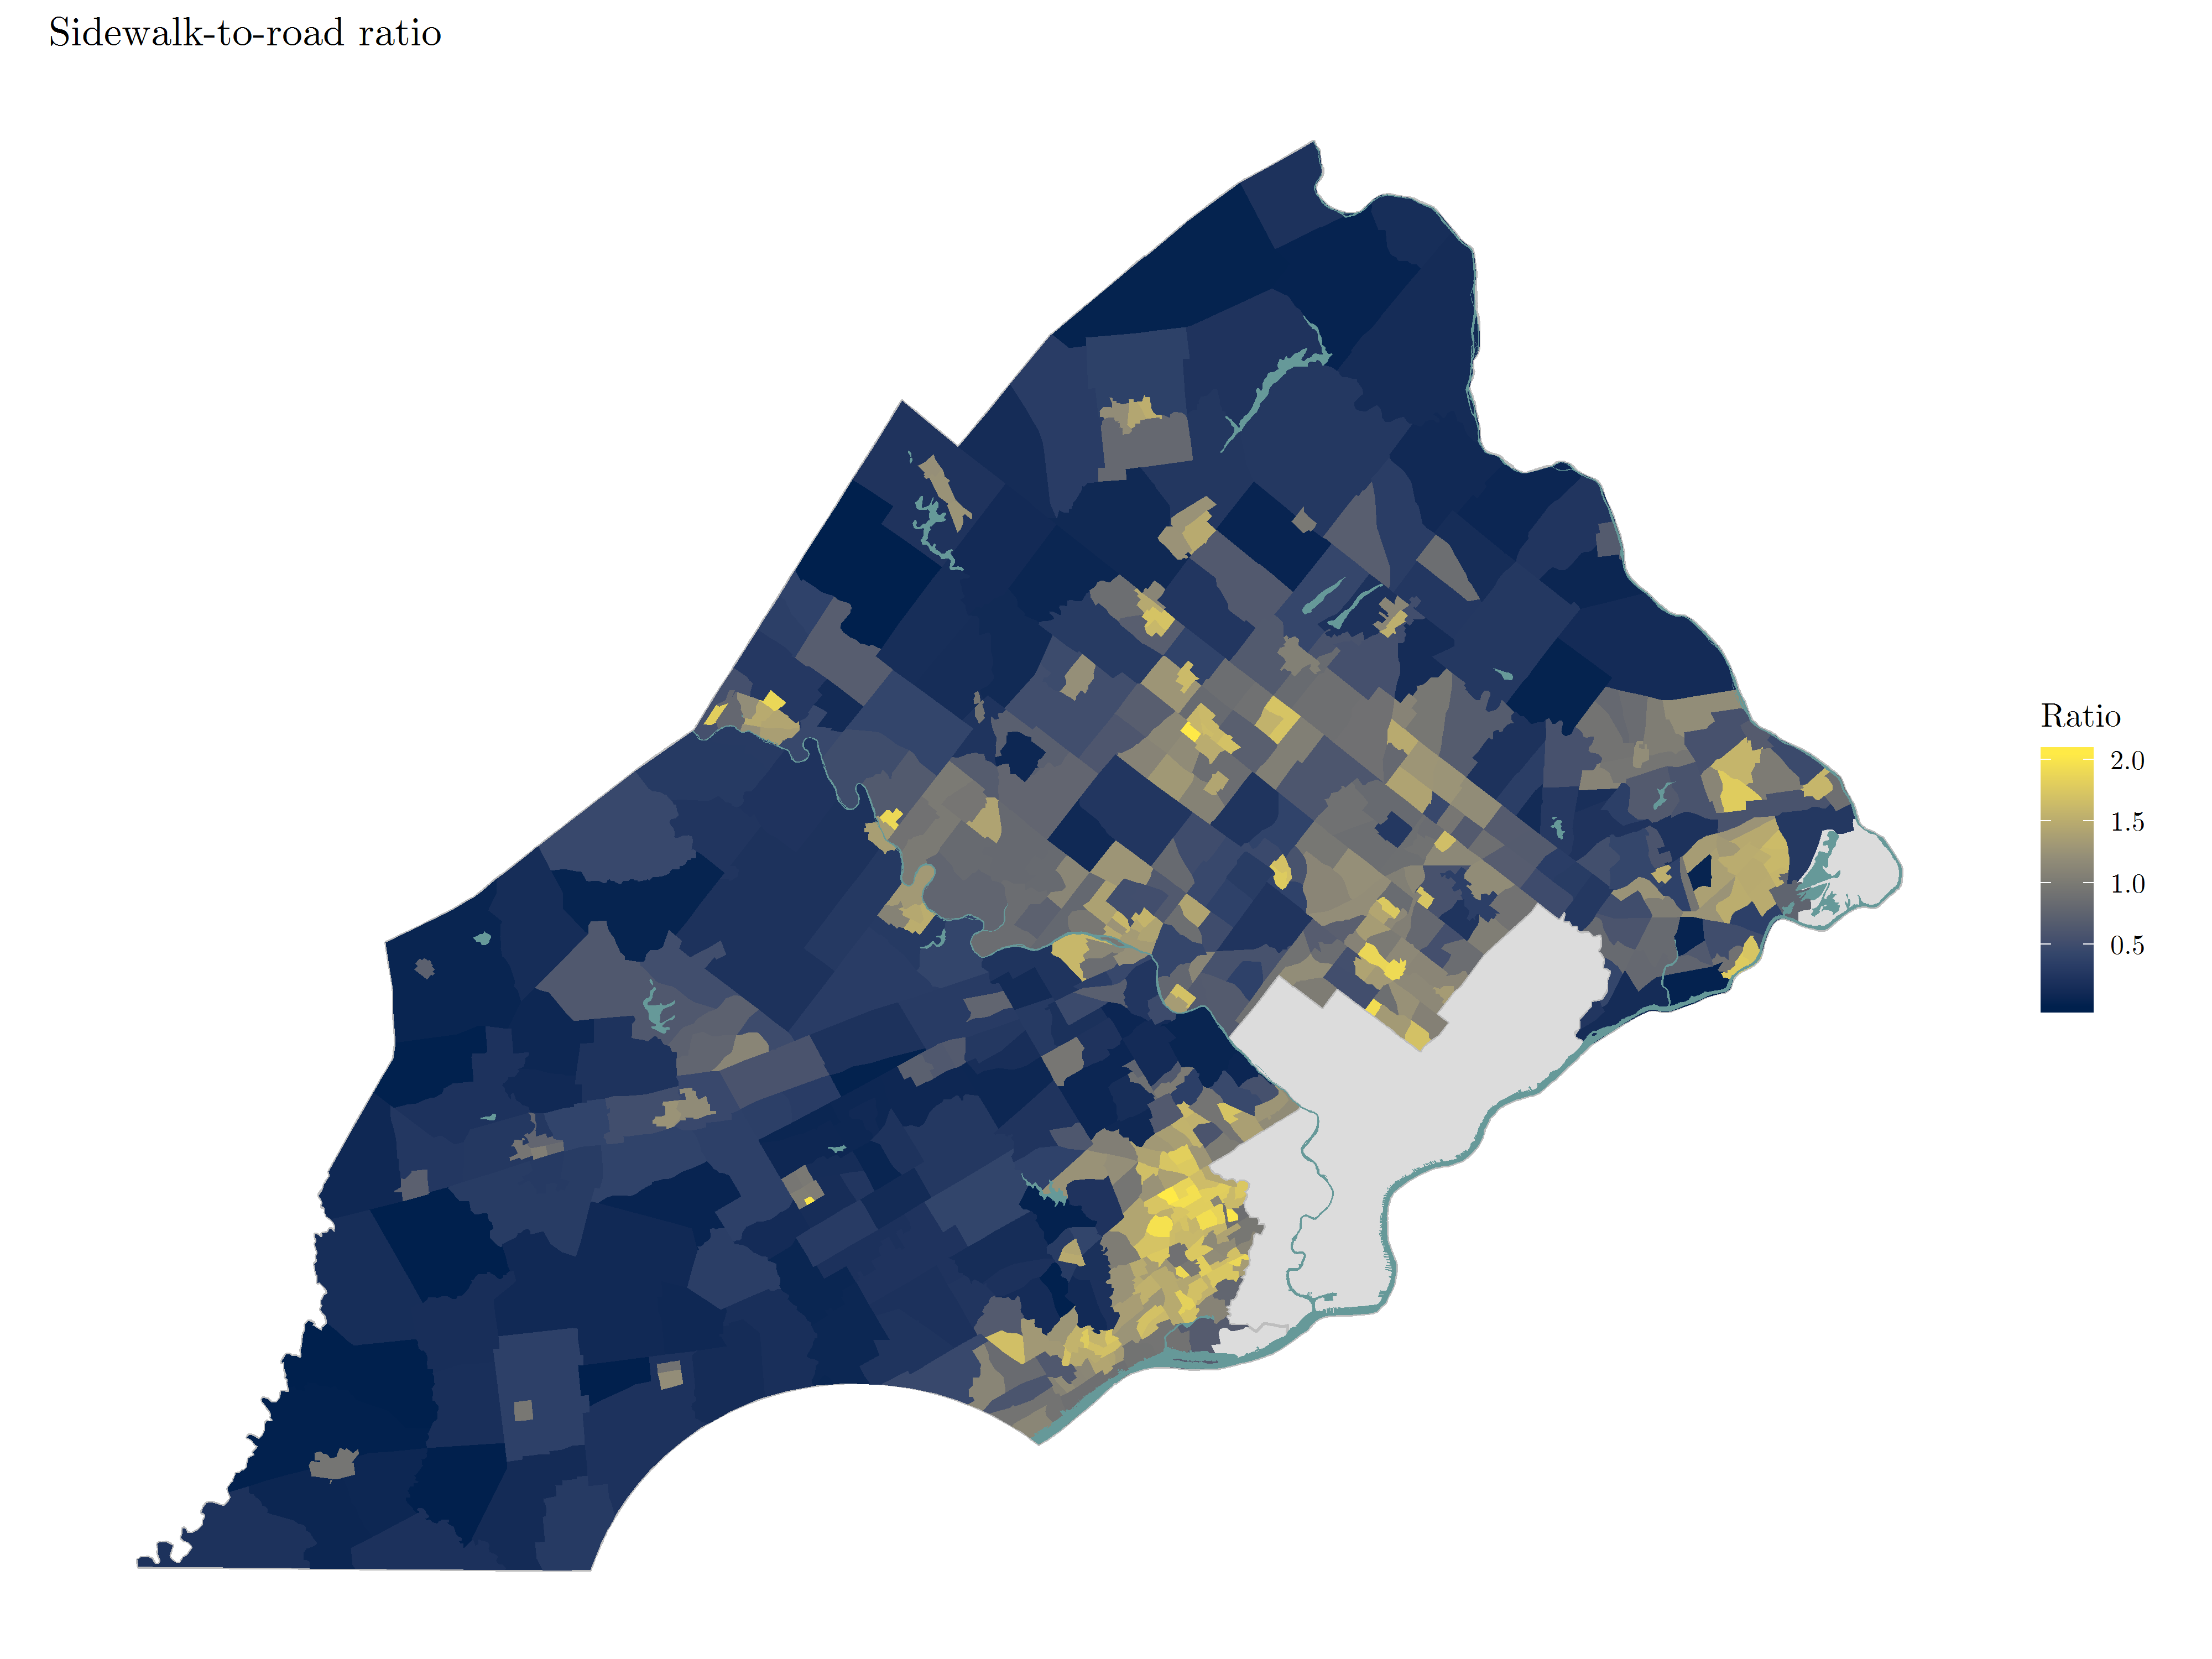
\includegraphics[width = 9in]{srr.png}
	\caption{Sidewalk-to-road ratio for the suburban PA counties. A ratio of 2 indicates full sidewalk coverage on both sides of every road. Limited access roads are removed from the centerline shapefile before processing.} \label{srr}
\end{sidewaysfigure}
\FloatBarrier

\subsubsection{Stepwise regressions}
Stepwise regressions identify the strongest correlates of pedestrian activity separately in Philadelphia and the four suburban Pennsylvania counties. Table~\ref{RegressionVariables} lists the variables used in regressions. Note the following assumptions and exclusions in regressions:

\begin{enumerate}[itemsep=-4pt]
	\item Census tracts with estimated total populations of less than 100 are excluded from regressions.
	\item Census tracts with estimated pedestrian densities exceeding $\left(\frac{30,000\:trips}{sq.\:mi.}\right)$ in the suburban counties and $\left(\frac{300,000\:trips}{sq.\:mi.}\right)$ in Philadelphia are excluded, as these observations are outliers.
	\item Many variables are highly positively skewed. If the skewness of a variable exceeds 1.5, we take the natural logarithm of the variable and use this value in regressions instead.
	\item Two separate sets of density measures are considered for Philadelphia and the suburban counties. In the City of Philadelphia, population and job density are combined into composite measures: ``people density,'' which is the sum of population and job density per census tract; and ``people interaction effect,'' which multiplies population by job density. Composite measures are considered in Philadelphia because the city has many mixed-use environments with around-the-clock pedestrian activity that cannot be accounted for by measuring only population or job density. In the suburban counties, population density and job density are considered as separate measures.
\end{enumerate}

\begin{table}
	\renewcommand*{\arraystretch}{1.4}
	\caption{Independent and dependent variables considered in regressions.}
	\label{RegressionVariables}
	\centering
	\begin{tabular}{|l c c|} 
		\hline
		\textbf{Variable} & \textbf{Philadelphia} & \textbf{Suburban Counties} \\
		\hline
		\multicolumn{3}{c}{\textit{Dependent}} \\
		\hline
		Estimated pedestrian density & \checkmark & \checkmark \\
		\hline
		\multicolumn{3}{c}{\textit{Independent}} \\
		\hline
		Population density & & \checkmark \\
		\hline
		Percentage of population enrolled in college & \checkmark & \checkmark \\
		\hline
		Job density & & \checkmark \\
		\hline
		Percentage of households below FPL & \checkmark & \checkmark \\
		\hline
		Transit activity density & \checkmark & \checkmark \\
		\hline
		Sidewalk density & \checkmark & \checkmark \\
		\hline
		Median household income, \$1000s & \checkmark & \checkmark \\
		\hline
		Percentage of zero-car households & \checkmark & \checkmark \\
		\hline
		Percentage of nonwhite residents & \checkmark & \checkmark \\
		\hline
		Number of pedestrian crashes in tract & \checkmark & \checkmark \\
		\hline
		Philadelphia Litter Index & \checkmark & \\
		\hline
		Land use mix & \checkmark & \checkmark \\
		\hline
		Sidewalk-to-road ratio & \checkmark & \checkmark \\
		\hline
		Road density & \checkmark & \checkmark \\
		\hline
		People density & \checkmark & \\
		\hline
		People interaction effect & \checkmark & \\
		\hline
	\end{tabular}
\end{table}

\textbf{Results: Philadelphia}
The percentage of college students and transit activity density are most highly correlated with expected pedestrian densities in the City of Philadelphia. These are the two variables used to create census tract sampling strata in Philadelphia. No other variable was found to be statistically significant. See Table~\ref{phila-reg} for regression results.

% Table created by stargazer v.5.2.2 by Marek Hlavac, Harvard University. E-mail: hlavac at fas.harvard.edu
% Date and time: Mon, Aug 05, 2019 - 8:40:39 AM
\begin{table}[!htbp] \centering 
	\caption{Estimated Pedestrian Density by Tract, Philadelphia} 
	\label{} 
	\begin{tabular}{@{\extracolsep{5pt}}lc} 
		\\[-1.8ex]\hline 
		\hline \\[-1.8ex] 
		\\[-1.8ex] & ln(Estimated Pedestrian Density by Tract) \\ 
		\hline \\[-1.8ex] 
		ln(Percentage college students) & 0.412$^{***}$ \\ 
		& (0.061) \\ 
		& \\ 
		Percentage residents below FPL & $-$0.002 \\ 
		& (0.004) \\ 
		& \\ 
		ln(Transit activity density) & 0.562$^{***}$ \\ 
		& (0.042) \\ 
		& \\ 
		Constant & 3.232$^{***}$ \\ 
		& (0.364) \\ 
		& \\ 
		\textit{N} & 370 \\ 
		R$^{2}$ & 0.423 \\ 
		Adjusted R$^{2}$ & 0.419 \\ 
		Residual Std. Error & 0.958 (df = 366) \\ 
		F Statistic & 89.531$^{***}$ (df = 3; 366) \\ 
		\hline 
		\hline \\[-1.8ex] 
		\textit{Notes:} & \multicolumn{1}{r}{$^{***}$Significant at the 1 percent level.} \\ 
		& \multicolumn{1}{r}{$^{**}$Significant at the 5 percent level.} \\ 
		& \multicolumn{1}{r}{$^{*}$Significant at the 10 percent level.} \\ 
	\end{tabular} 
\end{table} 

\textbf{Results: Four Suburban Counties}
The population density, percentage of college students, and road density are most highly correlated with expected pedestrian densities in the four suburban counties. These three variables are used to create census tract sampling strata in the four suburban counties. See Table~\ref{suburb-reg} for regression results.

% Table created by stargazer v.5.2.2 by Marek Hlavac, Harvard University. E-mail: hlavac at fas.harvard.edu
% Date and time: Wed, Feb 27, 2019 - 3:15:29 PM
\FloatBarrier
% Table created by stargazer v.5.2.2 by Marek Hlavac, Harvard University. E-mail: hlavac at fas.harvard.edu
% Date and time: Mon, Aug 05, 2019 - 8:39:58 AM
\begin{table}[!htbp] \centering 
	\caption{Estimated Pedestrian Density by Tract, Four Suburban Counties} 
	\label{} 
	\begin{tabular}{@{\extracolsep{5pt}}lc} 
		\\[-1.8ex]\hline 
		\hline \\[-1.8ex] 
		\\[-1.8ex] & ln(Estimated Pedestrian Density by Tract) \\ 
		\hline \\[-1.8ex] 
		ln(Population density) & 0.846$^{***}$ \\ 
		& (0.037) \\ 
		& \\ 
		ln(Percentage college students) & 0.314$^{***}$ \\ 
		& (0.030) \\ 
		& \\ 
		Road density & 0.031$^{***}$ \\ 
		& (0.005) \\ 
		& \\ 
		Constant & 5.020$^{***}$ \\ 
		& (0.074) \\ 
		& \\ 
		\textit{N} & 607 \\ 
		R$^{2}$ & 0.864 \\ 
		Adjusted R$^{2}$ & 0.864 \\ 
		Residual Std. Error & 0.435 (df = 603) \\ 
		F Statistic & 1,281.406$^{***}$ (df = 3; 603) \\ 
		\hline 
		\hline \\[-1.8ex] 
		\textit{Notes:} & \multicolumn{1}{r}{$^{***}$Significant at the 1 percent level.} \\ 
		& \multicolumn{1}{r}{$^{**}$Significant at the 5 percent level.} \\ 
		& \multicolumn{1}{r}{$^{*}$Significant at the 10 percent level.} \\ 
	\end{tabular} 
\end{table} 
\FloatBarrier

\subsubsection{Strata creation and distribution}
In Philadelphia, there are four possible sampling strata formed by the unique combinations of the census tract's share of college students and transit activity density classified into ``high'' and ``low'' values. See Table~\ref{PhilaStrata} for Philadelphia's four census tract sampling strata, where \textit{High} indicates a census tract's value greater than the median value and \textit{Low} indicates less than or equal to the median value. The column labeled \textbf{n} indicates the number of census tracts in each stratum.

\begin{table}
	\renewcommand*{\arraystretch}{1.4}
	\centering 
	\caption{Census tract sampling strata for the City of Philadelphia.} 
	\label{PhilaStrata} 
	\begin{tabular}{|c c c c|} 
		\hline 
		\textbf{Stratum} & \textbf{\% College Students} & \textbf{Transit Activity Density} & \textbf{n} \\
		\hline
		HH & High & High & 97 \\
		\hline
		HL & High & Low & 90 \\
		\hline
		LH & Low & High & 90 \\
		\hline
		LL & Low & Low & 97 \\
		\hline
	\end{tabular} 
\end{table}

\begin{figure}[!htbp]
	\centering
	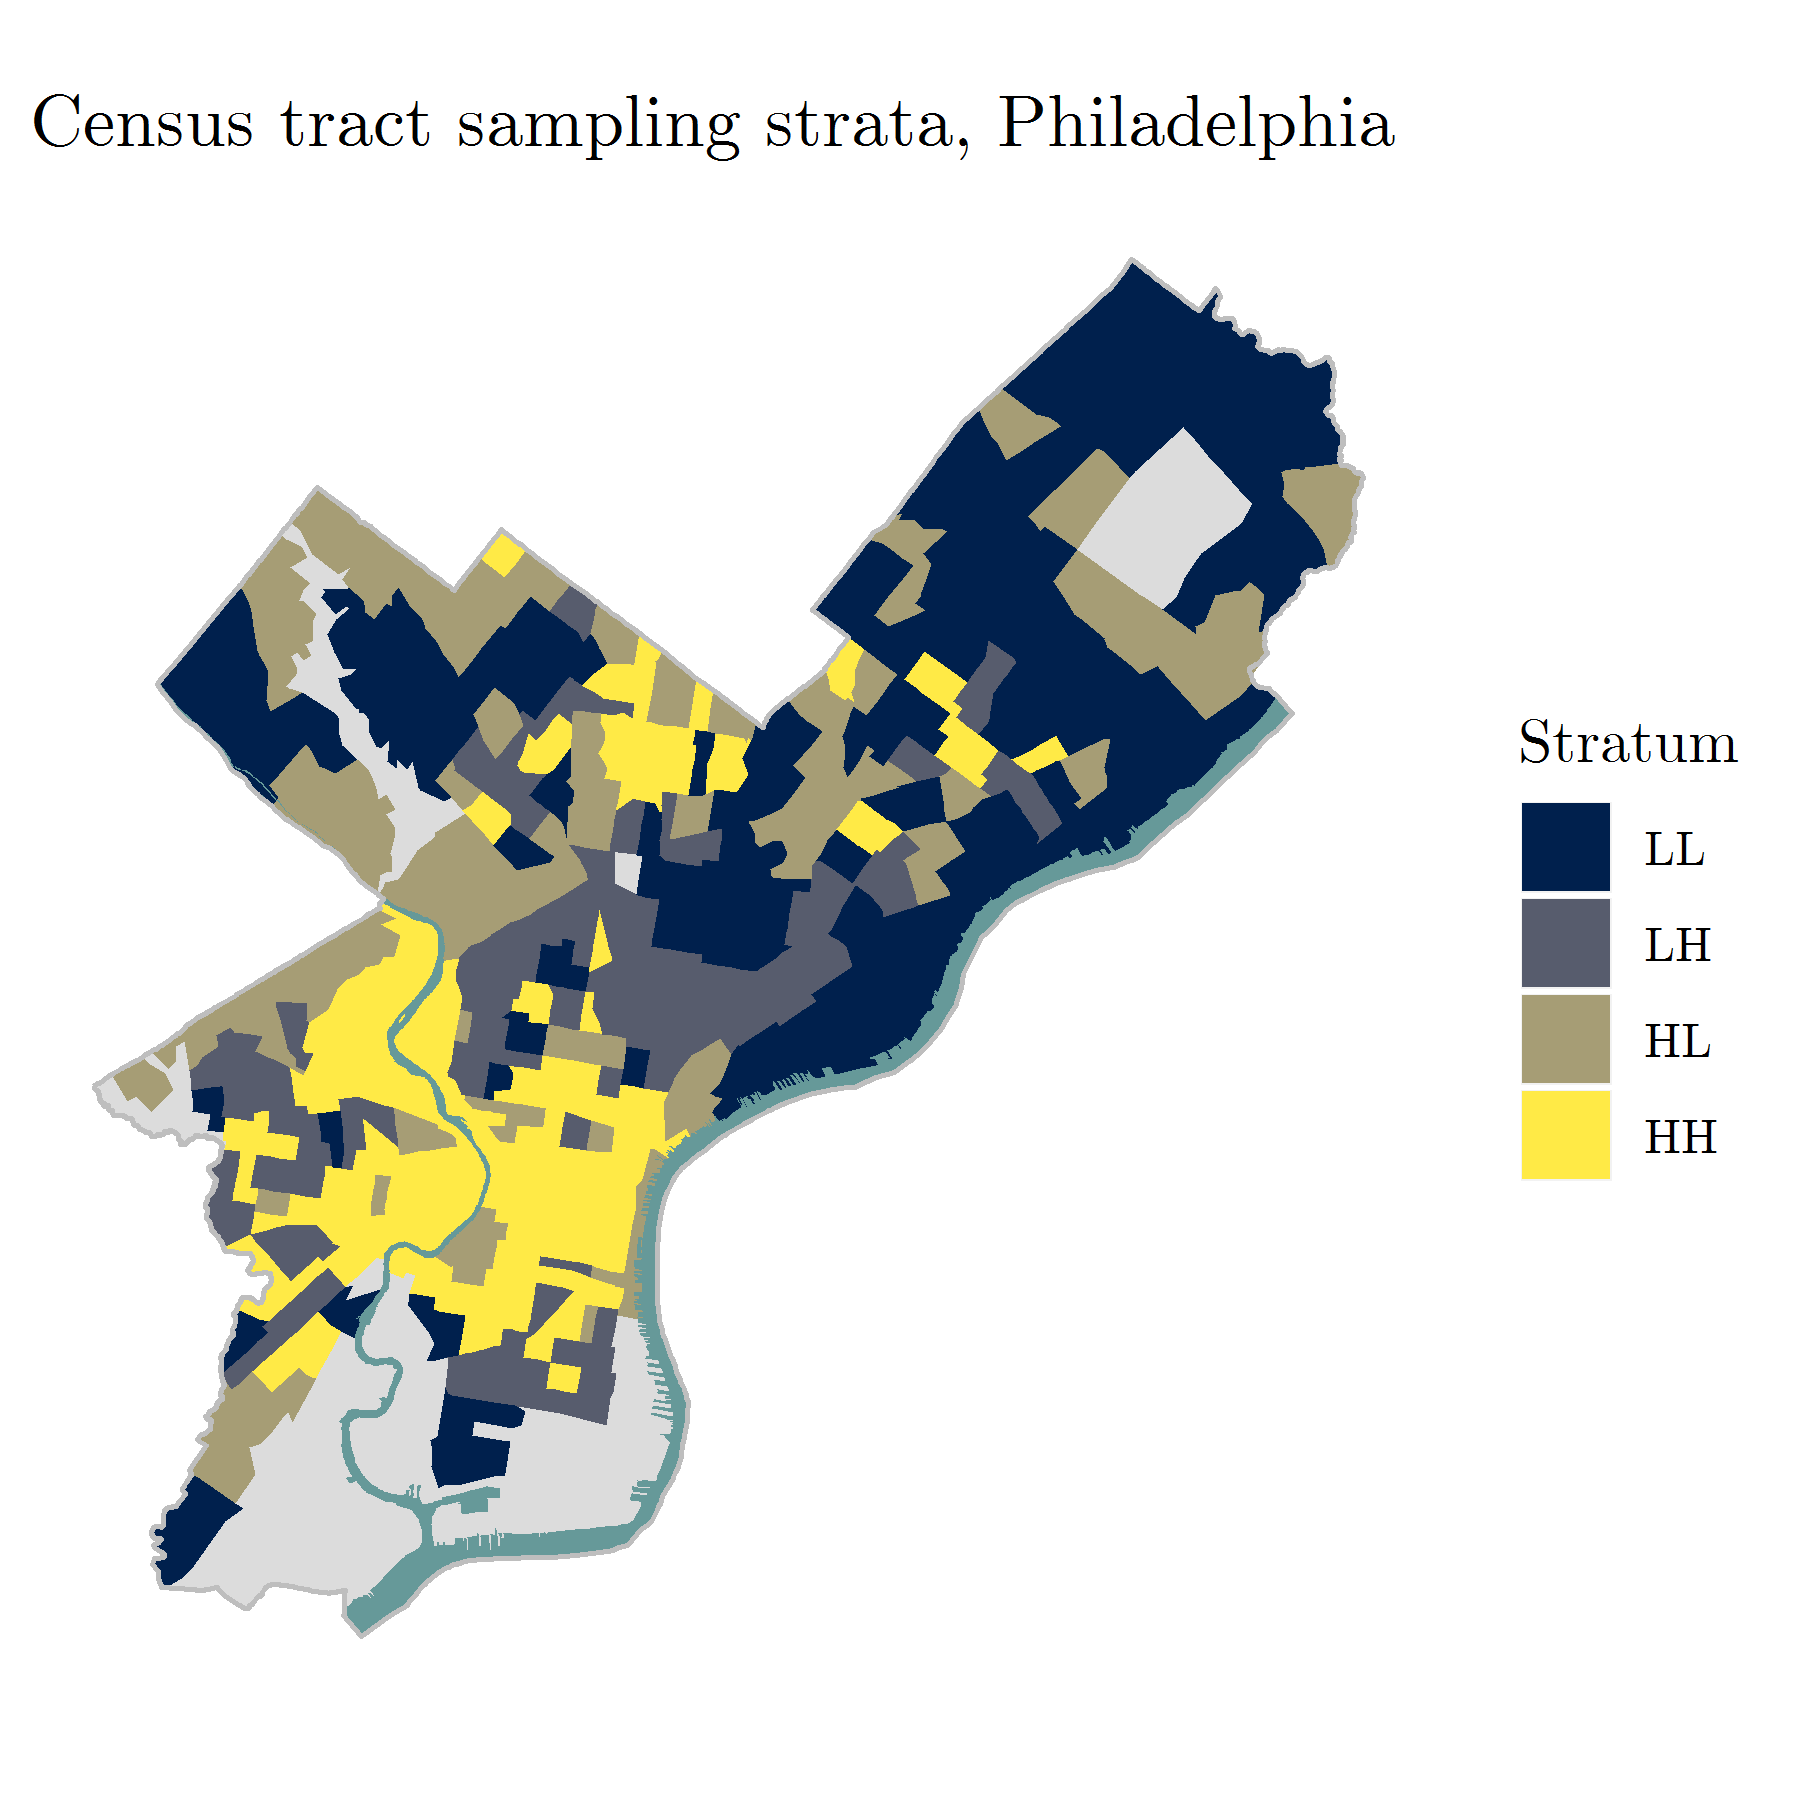
\includegraphics[width = 3.5in]{phila-areal.png}
	\caption{Census tract sampling strata in the City of Philadelphia.} \label{phila-areal}
\end{figure}

In the four suburban counties, there are eight possible sampling strata formed by the unique combinations of three variables classified into ``high'' and ``low'' values. See Table~\ref{SuburbStrata}, where \textit{High} indicates a census tract's value greater than the median value and \textit{Low} indicates less than or equal to the median value.

\begin{table}[!htbp]
	\renewcommand*{\arraystretch}{1.4}
	\centering 
	\caption{Census tract sampling strata for the four suburban counties.} 
	\label{SuburbStrata} 
	\begin{tabular}{|c c c c c|} 
		\hline 
		\textbf{Stratum} & \textbf{Population Density} & \textbf{\% College Students} & \textbf{Road Density} & \textbf{n} \\
		\hline
		HHH & High & High & High & 159 \\
		\hline
		HHL & High & High & Low & 17 \\
		\hline
		HLH & High & Low & High & 117 \\
		\hline
		LHH & Low & High & High & 16 \\
		\hline
		LLH & Low & Low & High & 14 \\
		\hline
		HLL & High & Low & Low & 13 \\
		\hline
		LHL & Low & High & Low & 114 \\
		\hline
		LLL & Low & Low & Low & 162 \\
		\hline
	\end{tabular} 
\end{table}

\FloatBarrier
\begin{sidewaysfigure}[h]
	\centering
	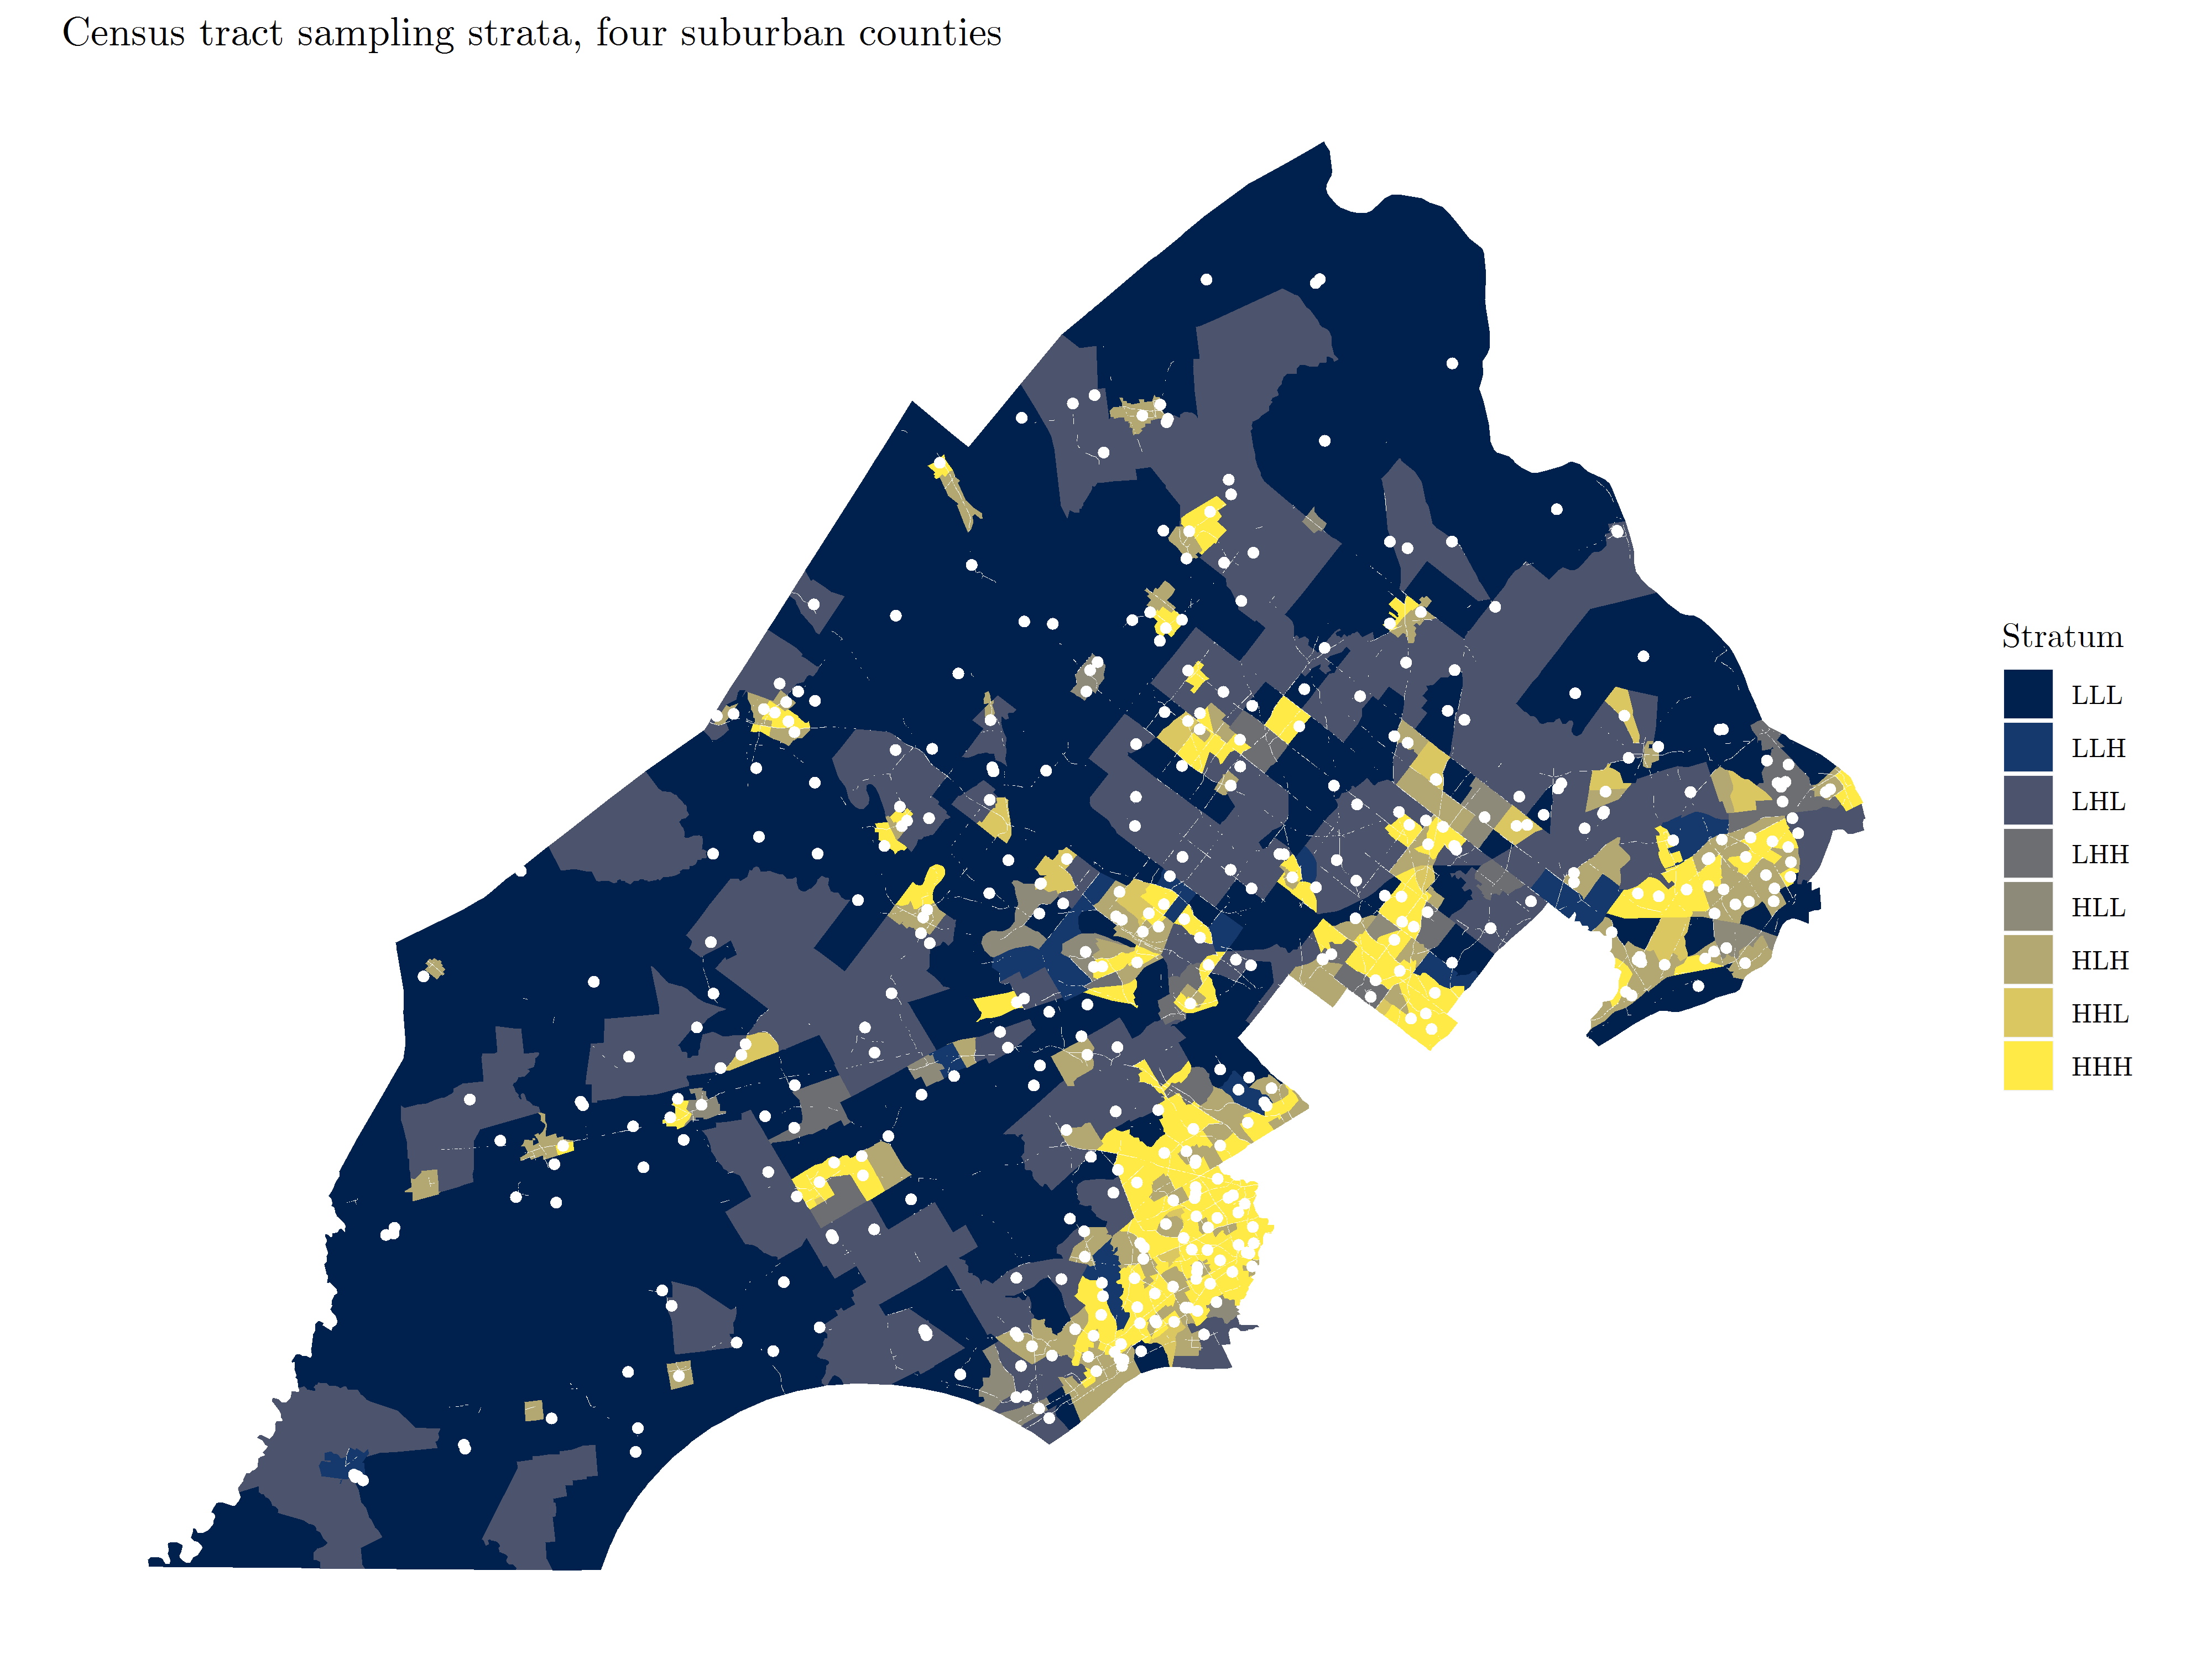
\includegraphics[width = 9in]{suburb-areal.png}
	\caption{Census tract sampling strata for the four suburban counties. The holes and small white lines in the map are areas where school and transit arterial strata have been erased from the census tract sampling strata.} \label{suburb-areal}
\end{sidewaysfigure}
\FloatBarrier

\subsection{Philadelphia transit arterial strata}
Philadelphia's transit arterial strata are comprised of high- and low-ridership segments of ``transit arterials.'' A ``transit arterial'' is defined as any road segment within 500 feet of a bus, trolley, or heavy rail stop or station. Many major roads in Philadelphia have transit stops or stations at regular intervals. These sampling strata capture differences in pedestrian activity between road segments with high or low ridership. \\

Developing transit arterial strata in the City of Philadelphia requires three major steps, including aggregating ridership data to account for nearby transit service, buffering road centerline features, and merging ridership and road data. \\

\textbf{Prepare ridership data}
Transit stops are often located in proximity to one another---for example, across the street---in dense urban environments. Sometimes a single transit stop is used by multiple bus or trolley lines. Because of the proximity of transit stops, there are often several stops and stations within reasonable walking distance of a given location. It is therefore insufficient to snap the ridership of a stop or station to the nearest road segment, because this ignores nearby transit. To capture the potential of nearby transit, ridership within 500 feet of each transit stop or station is aggregated and assigned to the observation. This process is repeated for all transit stops and stations in the City of Philadelphia. See Figure~\ref{stops} for a sample schematic of transit ridership at three stops and Table~\ref{sample-stops} for their corresponding ridership. \\

\begin{figure}[!htbp]
	\centering
	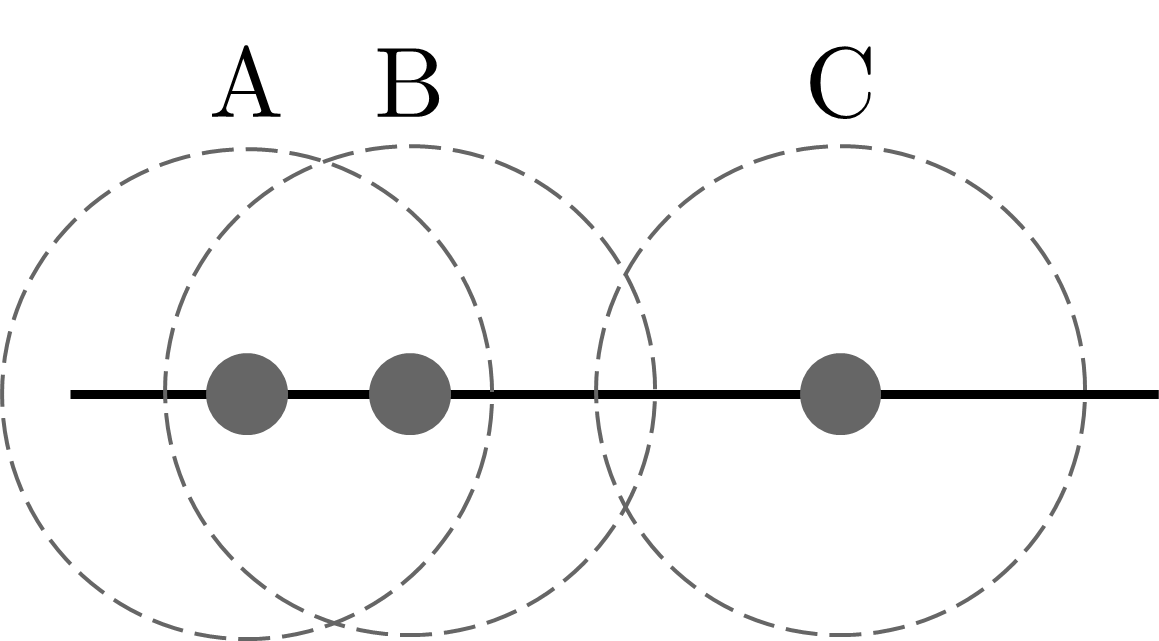
\includegraphics[width=3in]{stopdiag.png}
	\caption{Example of stop-level ridership buffers. Dots indicate transit stops, and dotted lines indicate a 500-foot buffer around each stop.} \label{stops}
\end{figure}

\begin{table}[!htbp]
	\renewcommand*{\arraystretch}{1.4}
	\centering 
	\caption{Aggregation of stop-level ridership. Notice that, though the buffers of B and C intersect, C's ridership is not assigned to B, and vice versa.} \label{sample-stops}
	\begin{tabular}{|c c c|} 
		\hline 
		\textbf{Stop} & \textbf{Original Ridership} & \textbf{Aggregated Ridership} \\
		\hline
		A & 225 & 240 \\
		\hline
		B & 15 & 240 \\
		\hline
		C & 45 & 45 \\
		\hline
	\end{tabular} 
\end{table}

\textbf{Prepare road centerline data}
The City of Philadelphia's road centerline data is available at a fine spatial resolution: generally, each road segment in the shapefile spans the length of one city block, intersection to intersection. Ramps, expressways, trails, walkway connectors, roads outside the city boundary, and small streets are removed from the road centerline file. Then, each segment is buffered by 50 feet to ensure that the aggregated ridership points can snap to their corresponding road segment. \\

\textbf{Merge ridership points with road segments}
Aggregated ridership points are spatially intersected with the buffered road segments. The resulting file is a crosswalk indicating which ridership points fall within each buffered road segment. \\

As seen in Figure~\ref{stops}, transit stops can be close to another and inherit each other's ridership attributes. To avoid counting the same transit riders multiple times, when multiple aggregated ridership points intersect with a single road segment, the segment is assigned the mean of these points. Figure~\ref{segments} shows the way aggregate ridership at Stops A, B, and C is snapped to segments. In this example, the darker segment receives a ridership of $\frac{\left(240 + 240\right)}{2} = 240$, and the lighter segment receives a ridership of 45.

\begin{figure}[!htbp]
	\centering
	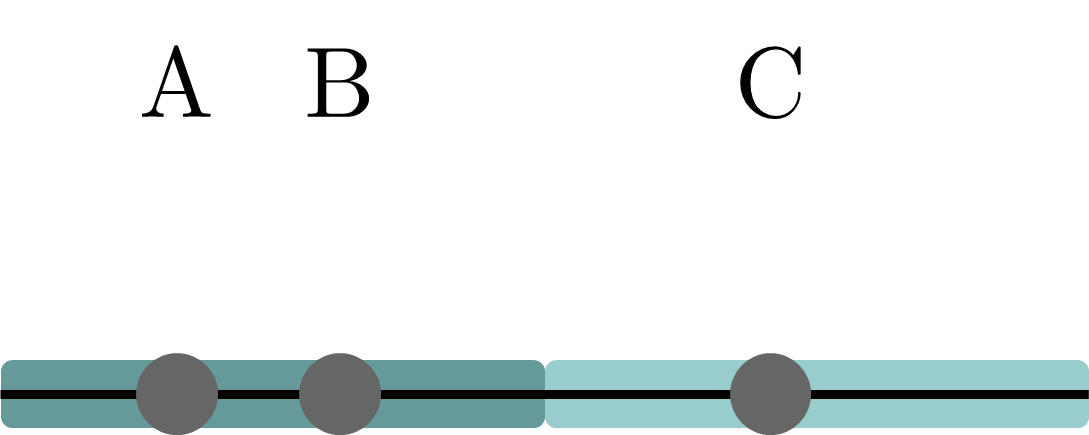
\includegraphics[width=3in]{stopdiagsegmentized.png}
	\caption{Assignment of aggregated stop-level ridership to buffered road segments.} \label{segments}
\end{figure}

\textbf{Determine high- and low-transit ridership segments.} Not every segment in the Philadelphia centerline file ($n = 24,572$ excluding ramps, expressways, etc.) is located within 500 feet of a transit stop. When this is the case, the record is not eligible for consideration as a transit arterial. This leaves 11,266 remaining road segments with ridership records. The road segments are split into high- and low-transit ridership segments based on the median ridership of 296.15. See Figure~\ref{phila-arterials} for the classification of high- and low-transit arterial segments in Center City Philadelphia.

\begin{figure}[!htbp]
	\centering
	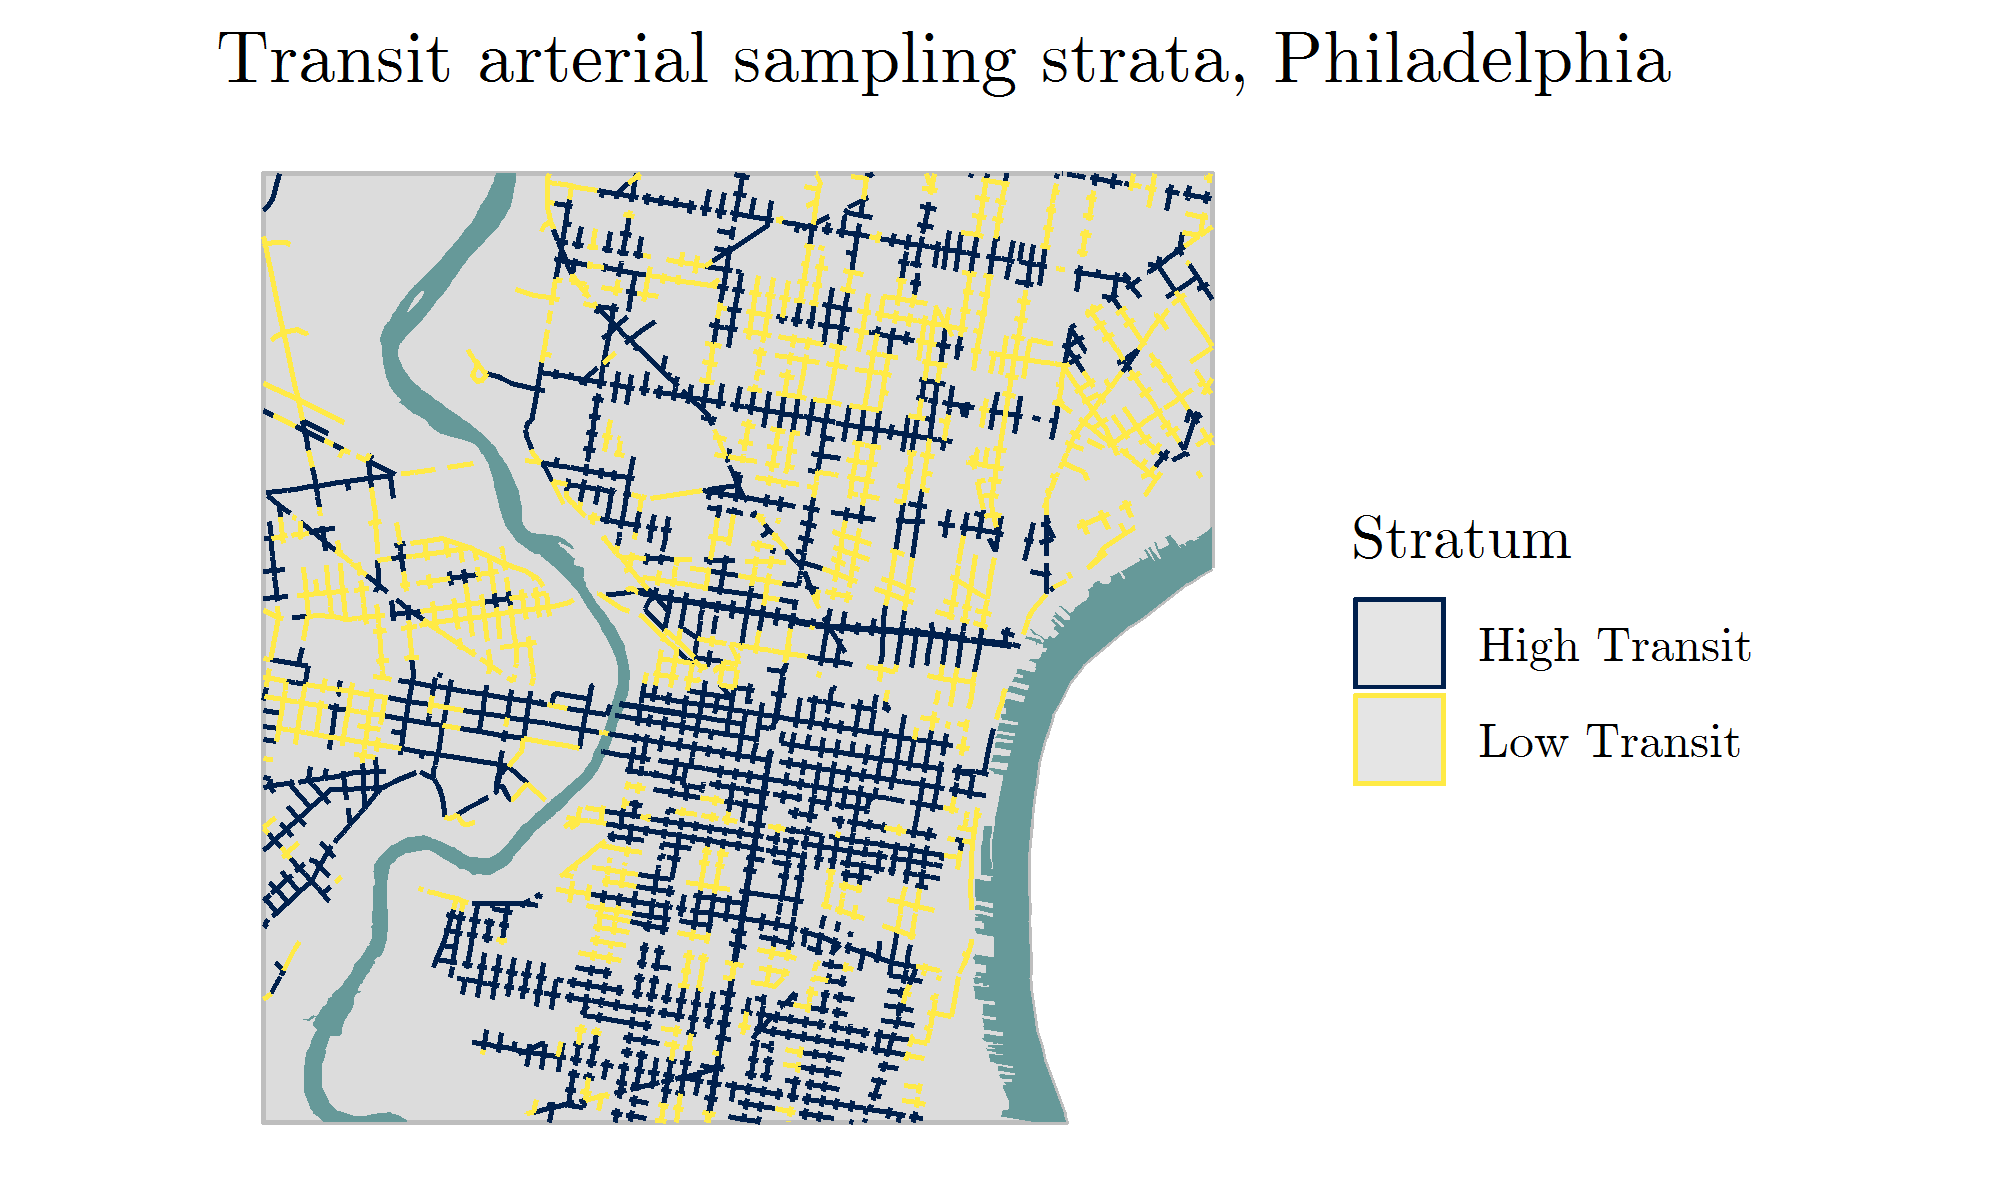
\includegraphics[width=5in]{phila-arterial.png}
	\caption{High- and low-ridership segments in Center City Philadelphia.} \label{phila-arterials}
\end{figure}

\subsection{Suburban transit arterial strata}
The transit arterial strata in the suburbs are comprised of ``transit arterials'' and ``non-transit arterials'' indicating the presence or absence of nearby transit service. Transit arterials are major and minor arterial segments with at least one transit stop within 0.25 miles; non-transit arterials are arterial segments farther than 0.25 miles from the nearest transit stop. Arterial segments must have sidewalk on at least one side of the road to be included in the sampling strata. \\

Creating the transit arterial strata requires extensive geoprocessing, including cutting the input road shapefile to eligible segments, slicing each remaining road segment into smaller segments of roughly equal length, and determining whether each segment is located near transit. \\ 

\textbf{Prepare functional class data}
Subset major and minor arterial records from the Pennsylvania functional class shapefile. Because the functional class file is not a centerline file, select only one side of the road for all two-way records. Cut the functional class shapefile extent to buffered sidewalks. Only arterial segments longer than 500 feet and located within 100 feet of a sidewalk are eligible for selection as a transit or non-transit arterial. \\

\textbf{Segmentize functional class records}
The functional class shapefile has some long road segments. 45 of 966 records are longer than two miles, and the longest record is 10.6 miles. It would be useless to suggest placing a pedestrian counter ``somewhere along'' the span of a 10-mile road segment. Each functional class segment is divided into smaller segments in a five-step process described below and shown for a single record in Figures~\ref{segmentize1} and~\ref{segmentize2}. While each line must be segmentized individually in Steps A through C, as shown in Figure~\ref{segmentize1}, it is more computationally efficient to apply Steps D through F, as shown in Figure~\ref{segmentize2} to the entire field of sample points exported from Step C.

\begin{enumerate}[A., itemsep=-4pt]
	\item Original functional class record for a single road.
	\item Drop a sample point at the beginning, every vertex, every 0.25 miles along straight stretches, and the end of the record using the \texttt{R} and PostGIS function \texttt{st\_segmentize}. Because a sample point is dropped at every vertex, some records can have hundreds of extra sample points.
	\item Iteratively compute the distance between consecutive points and filter out those that are less than 0.125 miles away.
	\item After creating a field of sample points that represent all line records in the functional class shapefile, determine which points are within 0.25 miles of a transit stop. Buffer all suburban transit stops and stations and overlay with the sample points. If a sample point intersects one or more transit stops and/or stations, then the variable \texttt{present} equals 1; otherwise, \texttt{present} equals 0.
	\item Convert the sample points to areal Voronoi polygons.
	\item Spatially intersect the Voronoi polygons and the original polyline shapefile. The result is a polyline shapefile divided into roughly 500-foot segments, each with a unique ID and indicating whether one or more transit stops are nearby. 
\end{enumerate}

\FloatBarrier
\begin{figure}[!htbp]
	\centering
	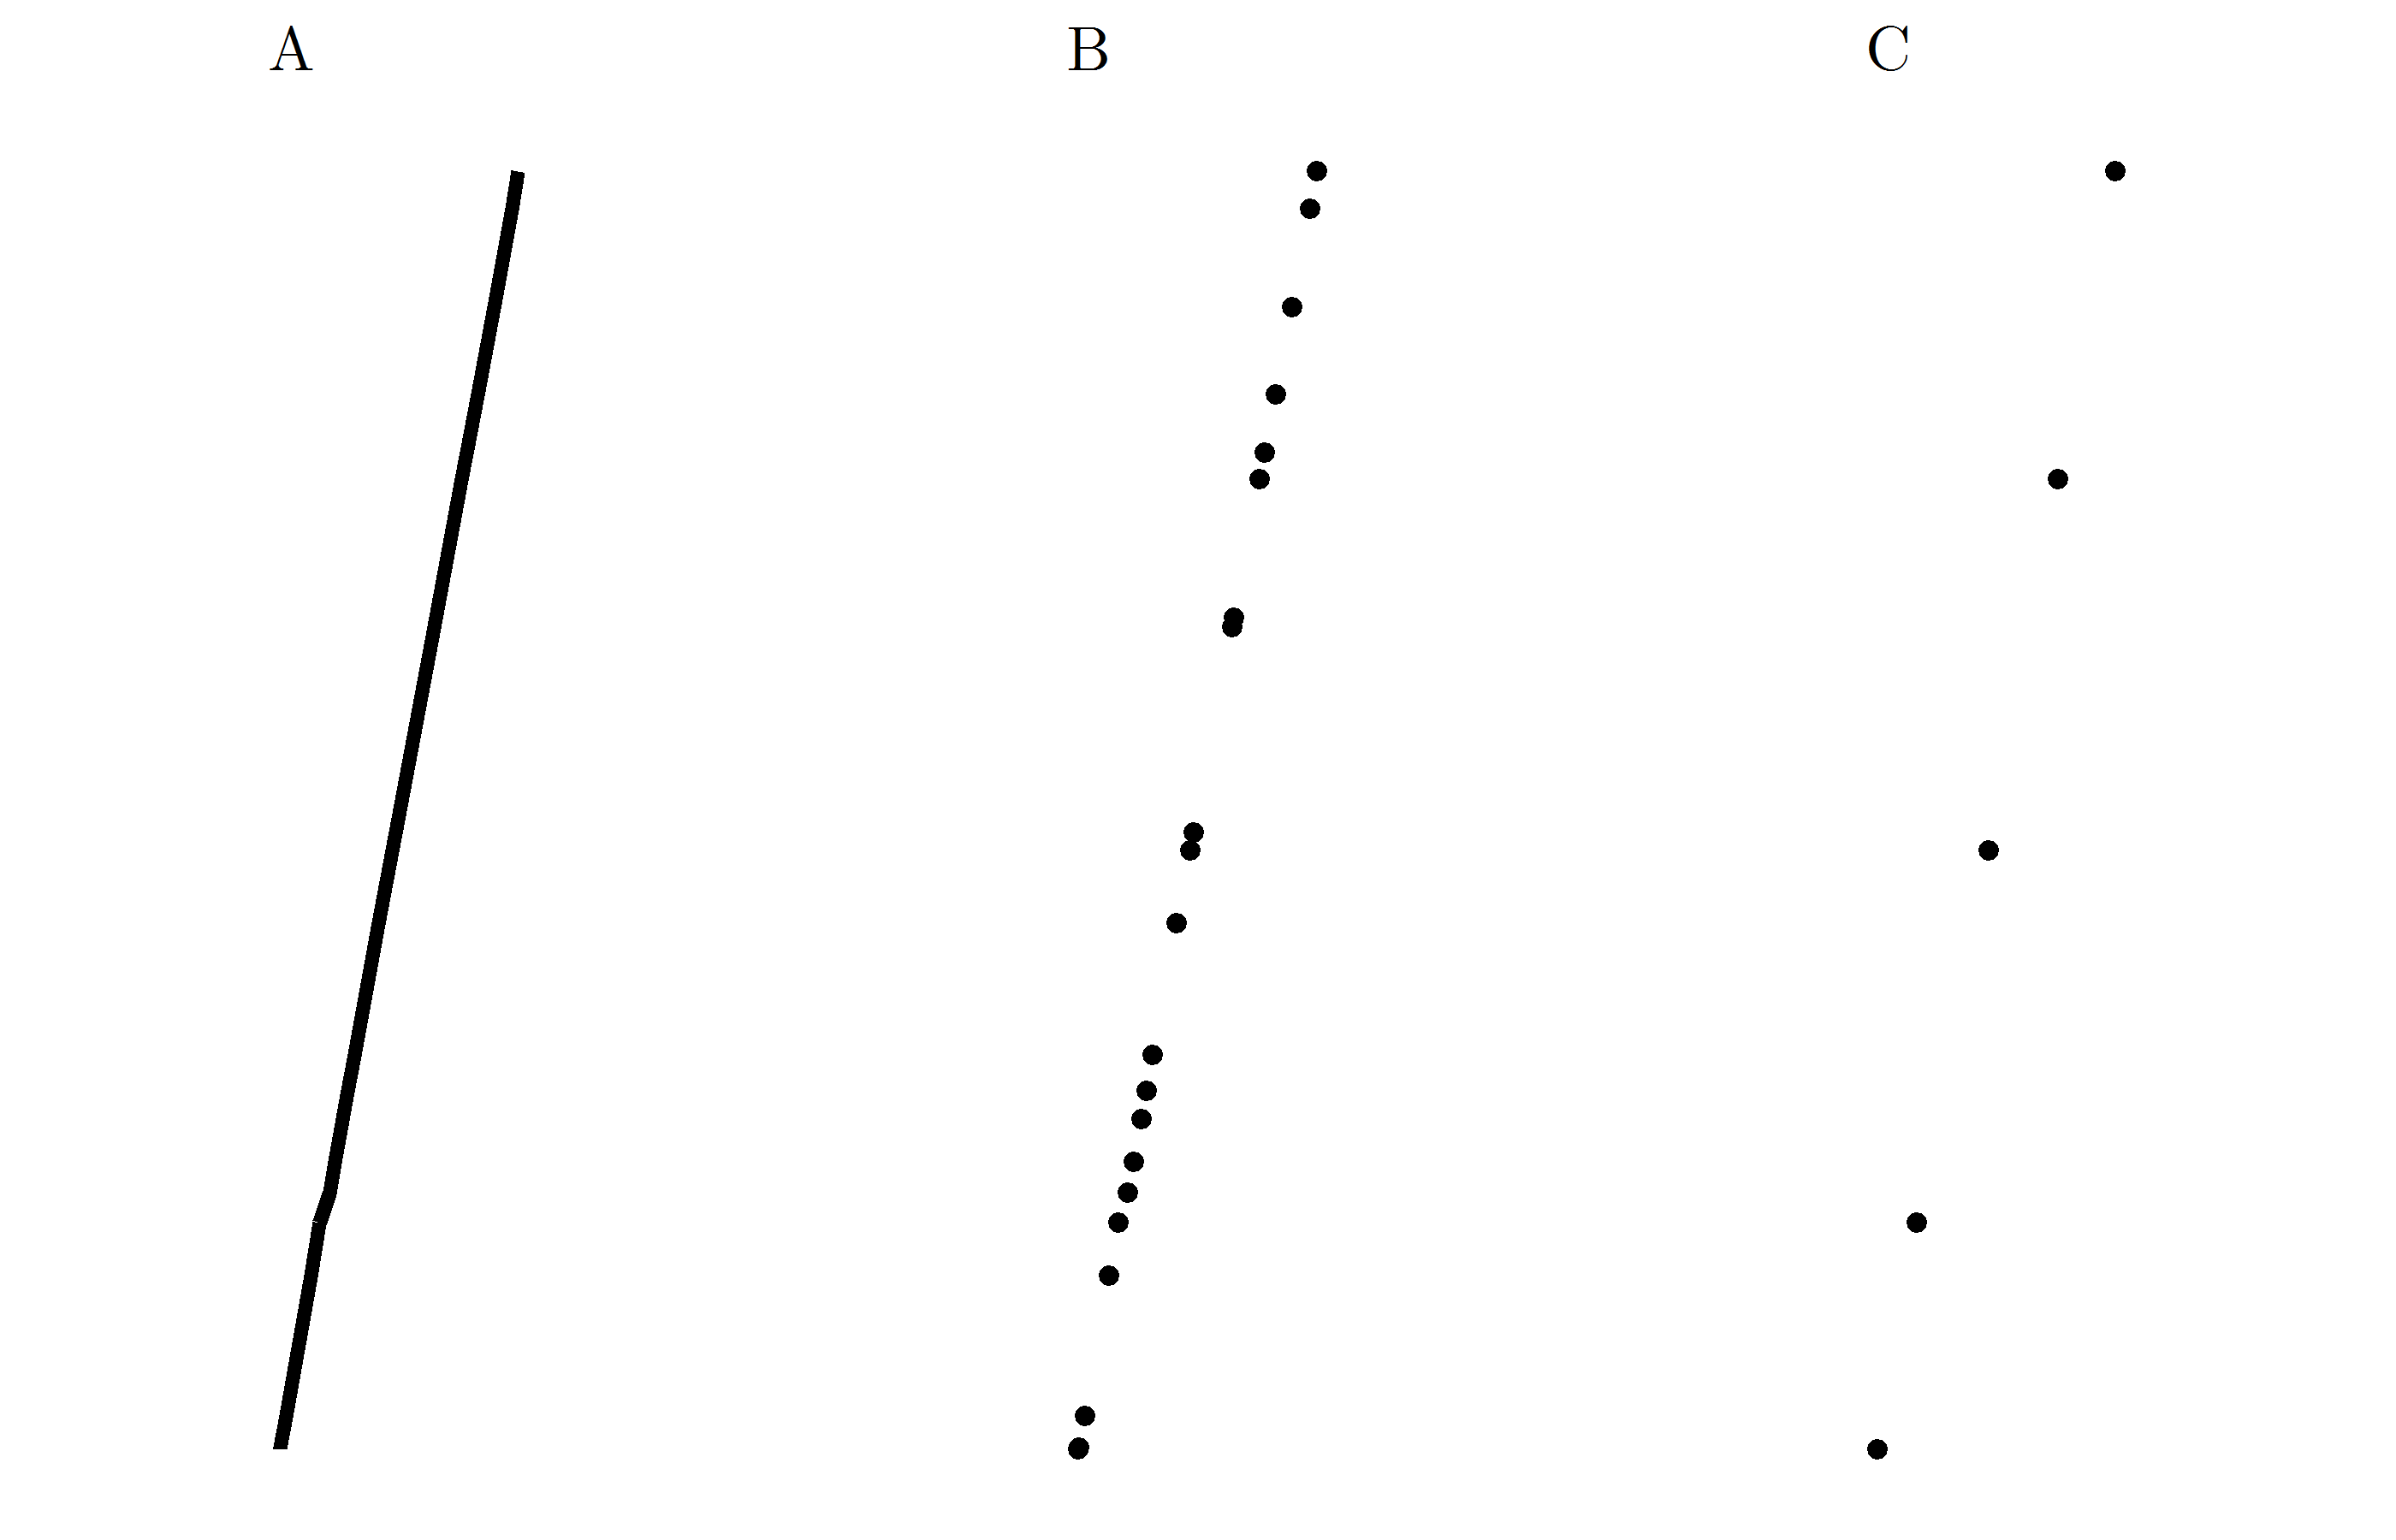
\includegraphics[width=5in]{segmentize-abc.png}
	\caption{Original functional class record (A), sample points (B), and filtered sample points (C).} \label{segmentize1}
\end{figure}
\FloatBarrier

\FloatBarrier
\begin{figure}[!htbp]
	\centering
	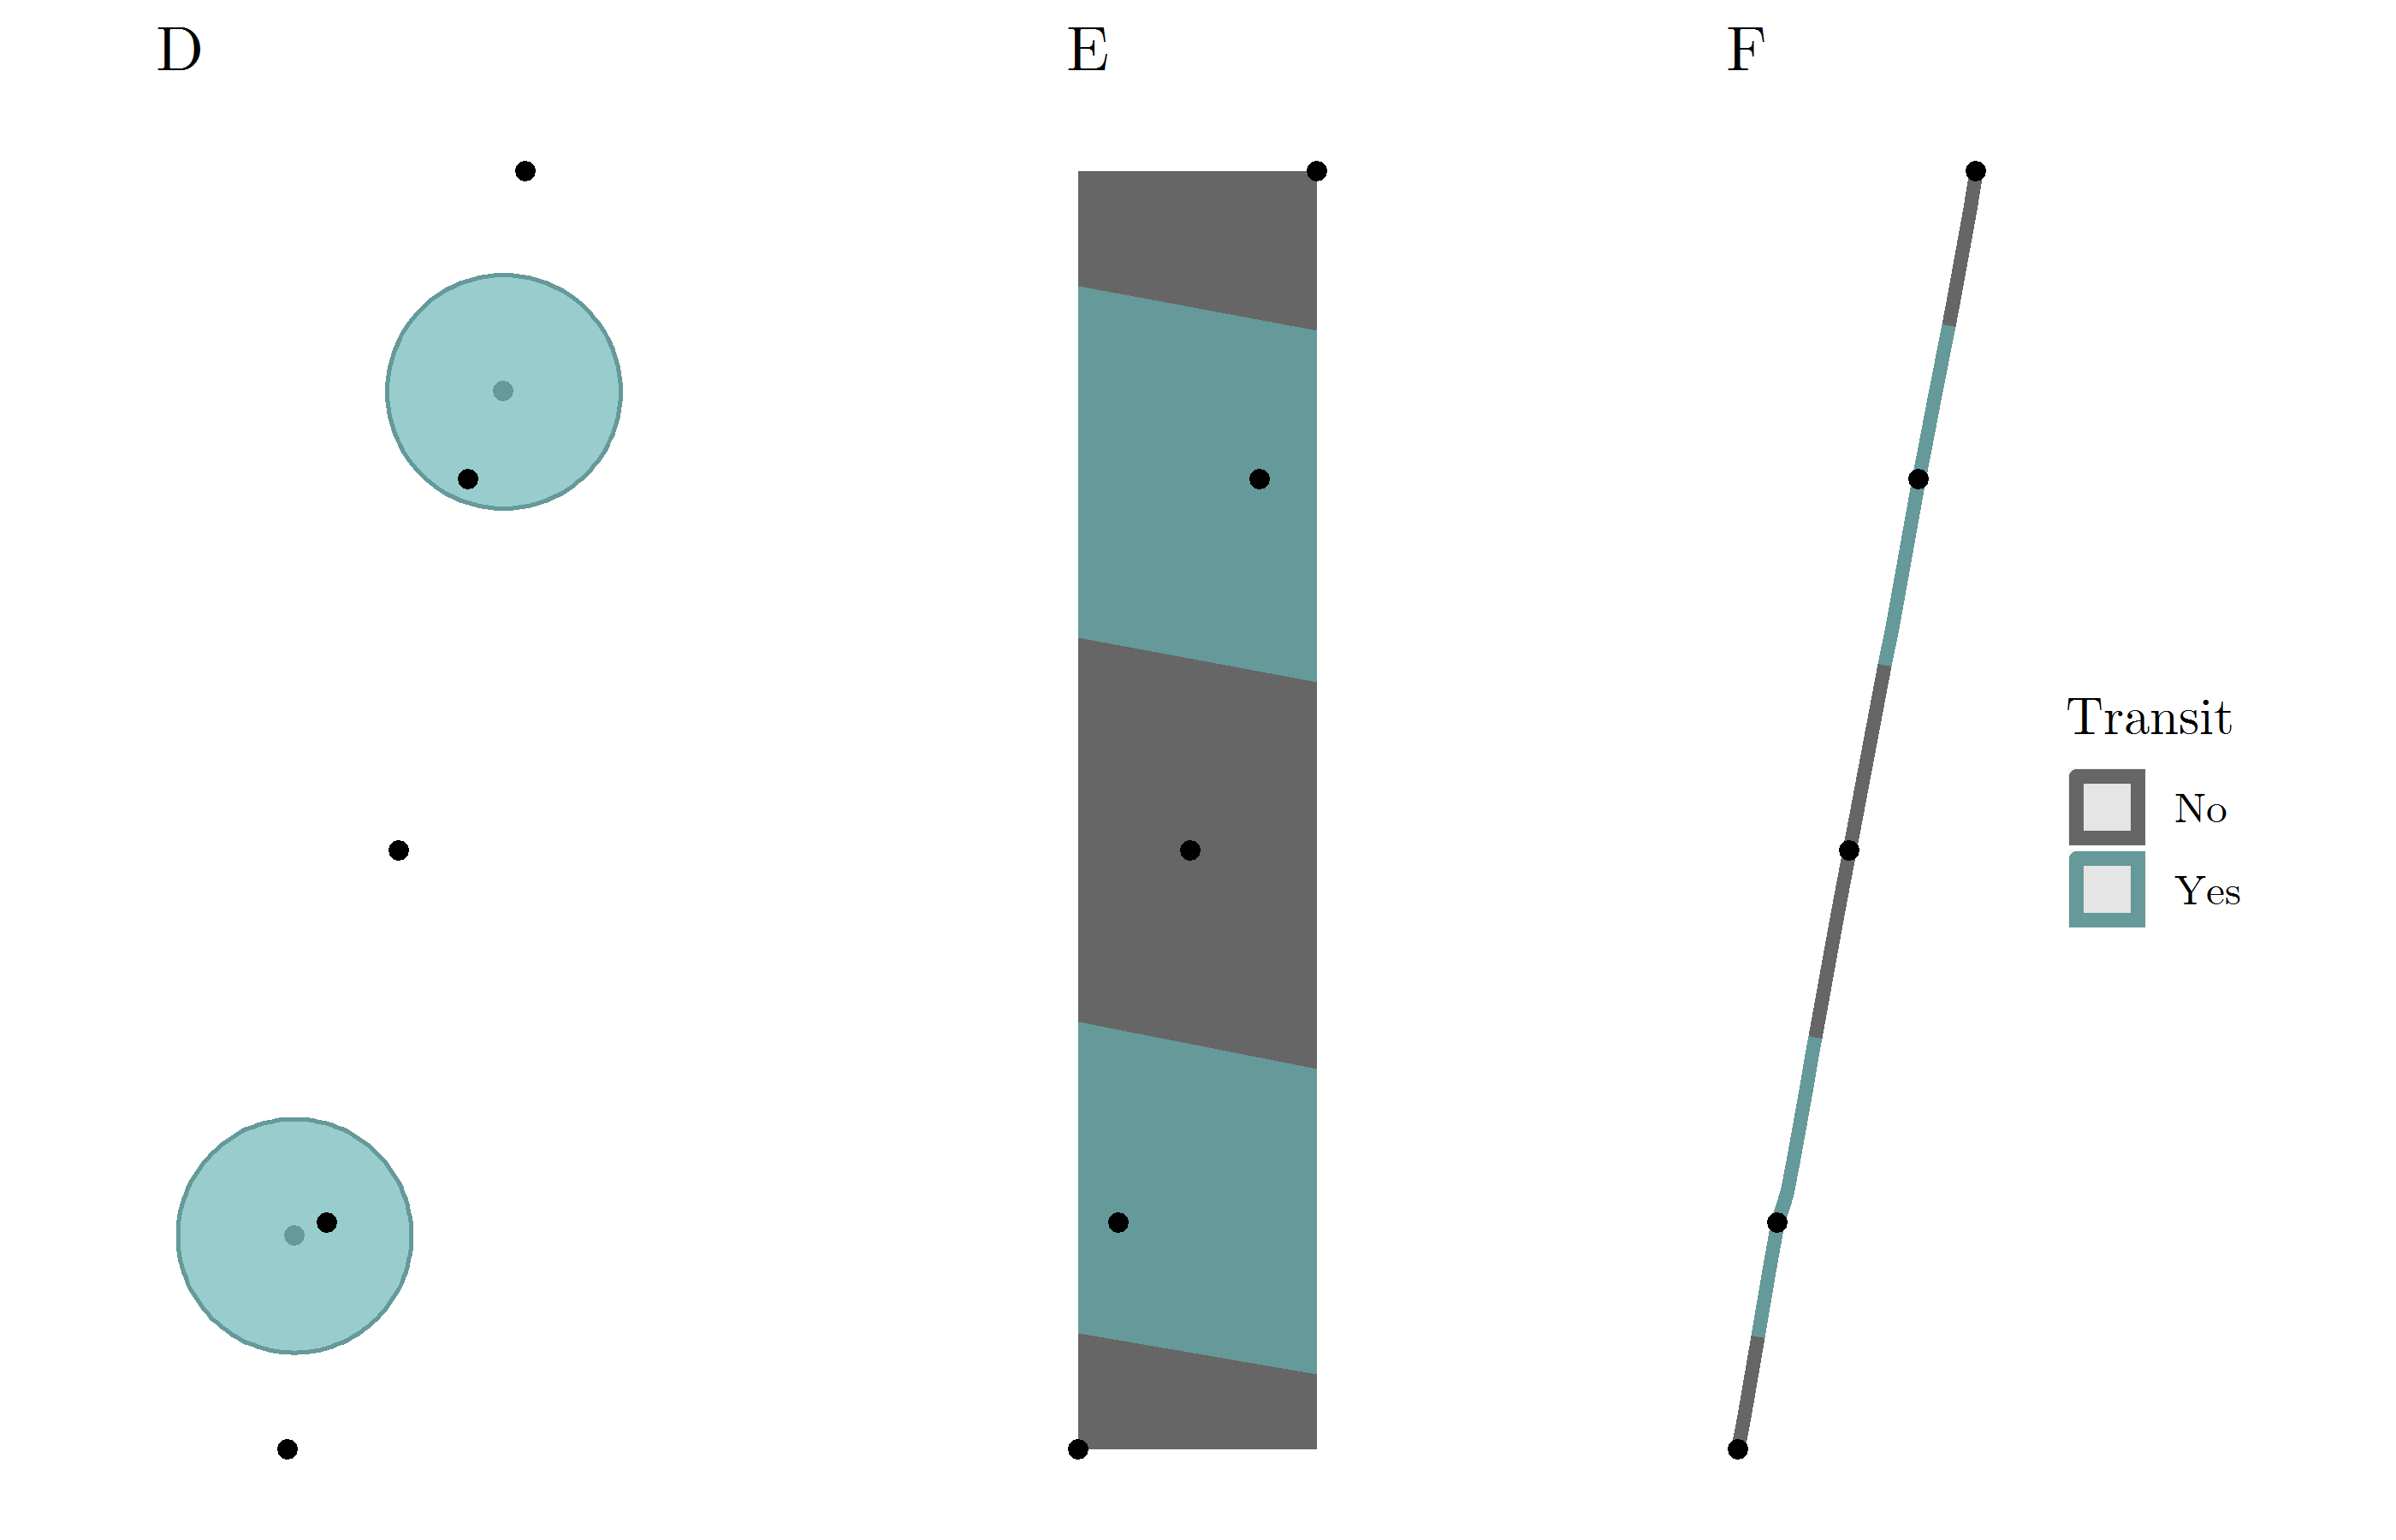
\includegraphics[width=5in]{segmentize-def.png}
	\caption{Functional class points intersected with transit stops (D), transformed into Voronoi polygons (E) and intersected with functional class polyline (F).} \label{segmentize2}
\end{figure}
\FloatBarrier

\subsection{Suburban school stratum}
The school stratum is comprised of public, charter, and magnet schools serving students in any of the grades K through 8. Each school is buffered by 0.25 miles to encompass the school grounds and surrounding area.

\section{Selection of count locations}
\label{sec:site-selection}
The site selection process includes two major steps. First, census tracts, arterial segments, and schools are randomly selected from among their sampling strata. Once these observations are selected, the physical attributes of each selected observation must be individually inspected to identify a location for pedestrian counting. In rare instances, the selected observation has no location with the proper specifications to conduct a count, requiring re-selection of another observation from the same sampling stratum. See 

\subsection{Suburban sampling strata}
While the primary goal of the stratified sampling scheme is to select a set of representative count locations, a secondary goal is to ensure a roughly equal distribution of count locations among the four suburban counties. This secondary goal requires additional steps in the selection process, which are outlined as \textit{rules} and \textit{exceptions}. See Script \href{https://github.com/addisonlarson/ped_counts/blob/master/6\_tract\_selector.R}{\texttt{6\_tract\_selector.R}}.\\

\subsubsection{Rules}

\textbf{Census tract sampling strata} Each census tract has two pieces of information: 1) its sampling stratum as determined in Section~\ref{sec:create-strata}; and 2) the county in which it falls. 10 counts are allocated to each of 8 sampling strata, meaning 80 counts distributed among four counties. Two census tracts are selected per sampling stratum per county, for a total of $\left(2\:counts \cdot 8\:strata \cdot 4\:counties = 64\:total\:counts\right)$ of 80 total census tract samples. This leaves 16 outstanding counts. For the outstanding counts, a ``pool'' of the remaining census tract counts is created. Delaware County has 0 LLH observations, so its two census tract counts are put into the pool as well. The pool includes 18 total counts: $\left(2\:counts \cdot 8\:strata + 2\:LLH \:counts = 18\:counts \right)$. Selection from the pool will be discussed later. \\

\textbf{Transit and non-transit arterial strata} 10 counts are selected from the transit and non-transit arterial strata, making 20 arterial strata counts in total. To ensure an even distribution of contexts, the transit and non-transit arterial observations are evenly distributed among the underlying census tract strata, i.e. $\left(1\:count \cdot 8\: strata = 8 \: counts\right)$. The remaining two counts per stratum are placed into the pool. \\

\textbf{School sampling stratum} 10 counts are selected from the school stratum. To ensure an even distribution of contexts, observations from the school stratum are evenly distributed among the underlying census tract strata, i.e. $\left(1\:count \cdot 8\: strata = 8 \: counts\right)$. The remaining two counts are placed into the pool. \\

\subsubsection{Exceptions}

\textbf{Pooled samples} Census tract sampling strata are not evenly distributed among the four suburban counties. See Table~\ref{SuburbStrataDistribution} for the count of census tracts by stratum and county. Because of the distribution of sampling strata among the counties, the remaining counts from the pool are allocated according to the share the stratum comprises within each county relative to the other counties. For example, LLL census tracts comprise 27\% of Bucks, 52\% of Chester, 7\% of Delaware, and 26\% of Montgomery County census tracts. The remaining LLL counts in the pool are allocated to Bucks and Chester Counties. See Table~\ref{SuburbStrataPooledFund} for the allocation of the remaining counts by county and sampling stratum. Montgomery County received three counts in the LHH stratum because it had several more LLH observations than the other counties.

\begin{table}[!htbp]
	\renewcommand*{\arraystretch}{1.4}
	\centering 
	\caption{Distribution of census tract sampling strata by county.} 
	\label{SuburbStrataDistribution} 
	\begin{tabular}{|c c c c c c |} 
		\hline 
		\textbf{Stratum} & \textbf{Bucks} & \textbf{Chester} & \textbf{Delaware} & \textbf{Montgomery} & \textbf{Total} \\
		\hline
		HHH & 19 & 11 & 74 & 55 & 159 \\
		\hline
		HHL & 6 & 2 & 3 & 6 & 17 \\
		\hline
		HLH & 34 & 13 & 32 & 38 & 117 \\
		\hline
		LHH & 3 & 3 & 0 & 10 & 16 \\
		\hline
		LLH & 3 & 2 & 2 & 7 & 14 \\
		\hline
		HLL & 4 & 2 & 3 & 4 & 13\\
		\hline
		LHL & 35 & 23 & 19 & 37 & 114 \\
		\hline
		LLL & 38 & 60 & 10 & 54 & 162 \\
		\hline
	\end{tabular} 
\end{table}

\begin{table}[!htbp]
	\renewcommand*{\arraystretch}{1.4}
	\centering 
	\caption{Allocation of remaining counts from the pool.} 
	\label{SuburbStrataPooledFund} 
	\begin{tabular}{|c c c c c |} 
		\hline 
		\textbf{Stratum} & \textbf{Bucks} & \textbf{Chester} & \textbf{Delaware} & \textbf{Montgomery} \\
		\hline
		HHH & & & \checkmark & \checkmark  \\
		\hline
		HHL & \checkmark & & \checkmark & \\
		\hline
		HLH & \checkmark & & & \checkmark \\
		\hline
		LHH & & \checkmark & & \checkmark \checkmark \checkmark \\
		\hline
		LLH & \checkmark & & & \checkmark \\
		\hline
		HLL & \checkmark & & \checkmark & \\
		\hline
		LHL & & \checkmark & \checkmark & \\
		\hline
		LLL & \checkmark & \checkmark & & \\
		\hline
		School & \checkmark & \checkmark & & \\
		\hline
		Transit & & \checkmark & \checkmark & \\
		\hline
		Non-Transit & & \checkmark & \checkmark & \\
		\hline
	\end{tabular} 
\end{table}

\subsubsection{Count locations}

\textbf{Census tract sampling strata} After selecting census tracts from the census tract sampling stratum, we contacted the planning departments of each suburban county with maps of the selected census tracts and guidelines for site selection. Each of these counties responded with a set of physical count locations. For more on this, see Section~\ref{sec:stakeholder-engagement}. \\

Two selected census tracts in Chester County were determined to have no sufficient locations for conducting counts. Census Tract 42045405000 in Chester City was dominated by several schools, which erased much of the tract's land area, and the Chester Transportation Center. The only suitable location in Census Tract 42045407000 in Chester Heights borough was inside a private apartment complex; it would be difficult to obtain permission to conduct a count here, and the count would likely only capture pedestrian patterns within the complex. These observations were replaced with other randomly selected observations in the same sampling strata within Chester County. \\

\textbf{Transit arterials, non-transit arterials, and schools} Count locations along selected transit and non-transit arterial observations were selected by DVRPC staff. The requirements for selecting a physical count location include the following:
\begin{itemize}[itemsep=-4pt]
	\item Sidewalk on at least one side of the selected arterial segment;
	\item A fixed object pointing away from the road to securely fasten the infrared pedestrian counting equipment;
	\item Reasonable distance away from places where people could be ``milling about,'' e.g. a bench along a downtown street;
	\item Reasonable distance away from mailboxes; and
	\item Nearest the bus stop with highest ridership if the transit arterial segment contains multiple bus stops.
\end{itemize}

\subsection{Philadelphia sampling strata}
\textbf{High- and low-transit arterial strata} 10 counts are selected from the high- and low-transit arterial strata, making 20 arterial strata counts in total. To ensure an even distribution of contexts, the transit and non-transit arterial observations are evenly distributed among the underlying census tract strata, i.e. $\left(1\:count \cdot 8\: strata = 8 \: counts\right)$. The remaining two counts per stratum are placed into the pool. \\

\subsubsection{Rules}

\textbf{Census tract sampling strata} 10 counts are allocated to each of 4 sampling strata, meaning 40 counts distributed among the city. \\

\textbf{High- and low-ridership transit streets strata} 10 counts are selected from high- and low-ridership -transit streets strata, making 20 streets strata counts in total. To ensure an even distribution of contexts, the high- and low-ridership observations are evenly distributed among the underlying census tract strata, i.e. $\left(1\:count \cdot 8\: strata = 8 \: counts\right)$. \\

\section{Correspondence with member governments}
\label{sec:stakeholder-engagement}
Because the study area for the cyclical pedestrian counting program spans five counties, DVRPC's member governments provide crucial input in selecting count locations. The list below summarizes inputs from local officials on each sampling strata type:

\begin{itemize}
	\item \textbf{Census tract sampling strata} Member governments select the count location, with the request that the selected location be representative of pedestrian patterns in the census tract overall. See Figure~\ref{corresp-3} for an example of a letter sent to county officials regarding site selection and Figure~\ref{corresp-4} for an example of an accompanying map.
	\item \textbf{Transit and non-transit arterial sampling strata} DVRPC staff select the count locations, and member governments verify whether any transportation or development projects are expected to occur near the locations. See Figure~\ref{corresp-1} for an example of a letter sent to county officials regarding site verification and Figure~\ref{corresp-2} for an example of an accompanying map.
	\item \textbf{School sampling strata} DVRPC staff select the count locations, and member governments verify whether any transportation or development projects are expected to occur near the locations.
\end{itemize}

\FloatBarrier
\begin{figure}[!htbp]
	\centering
	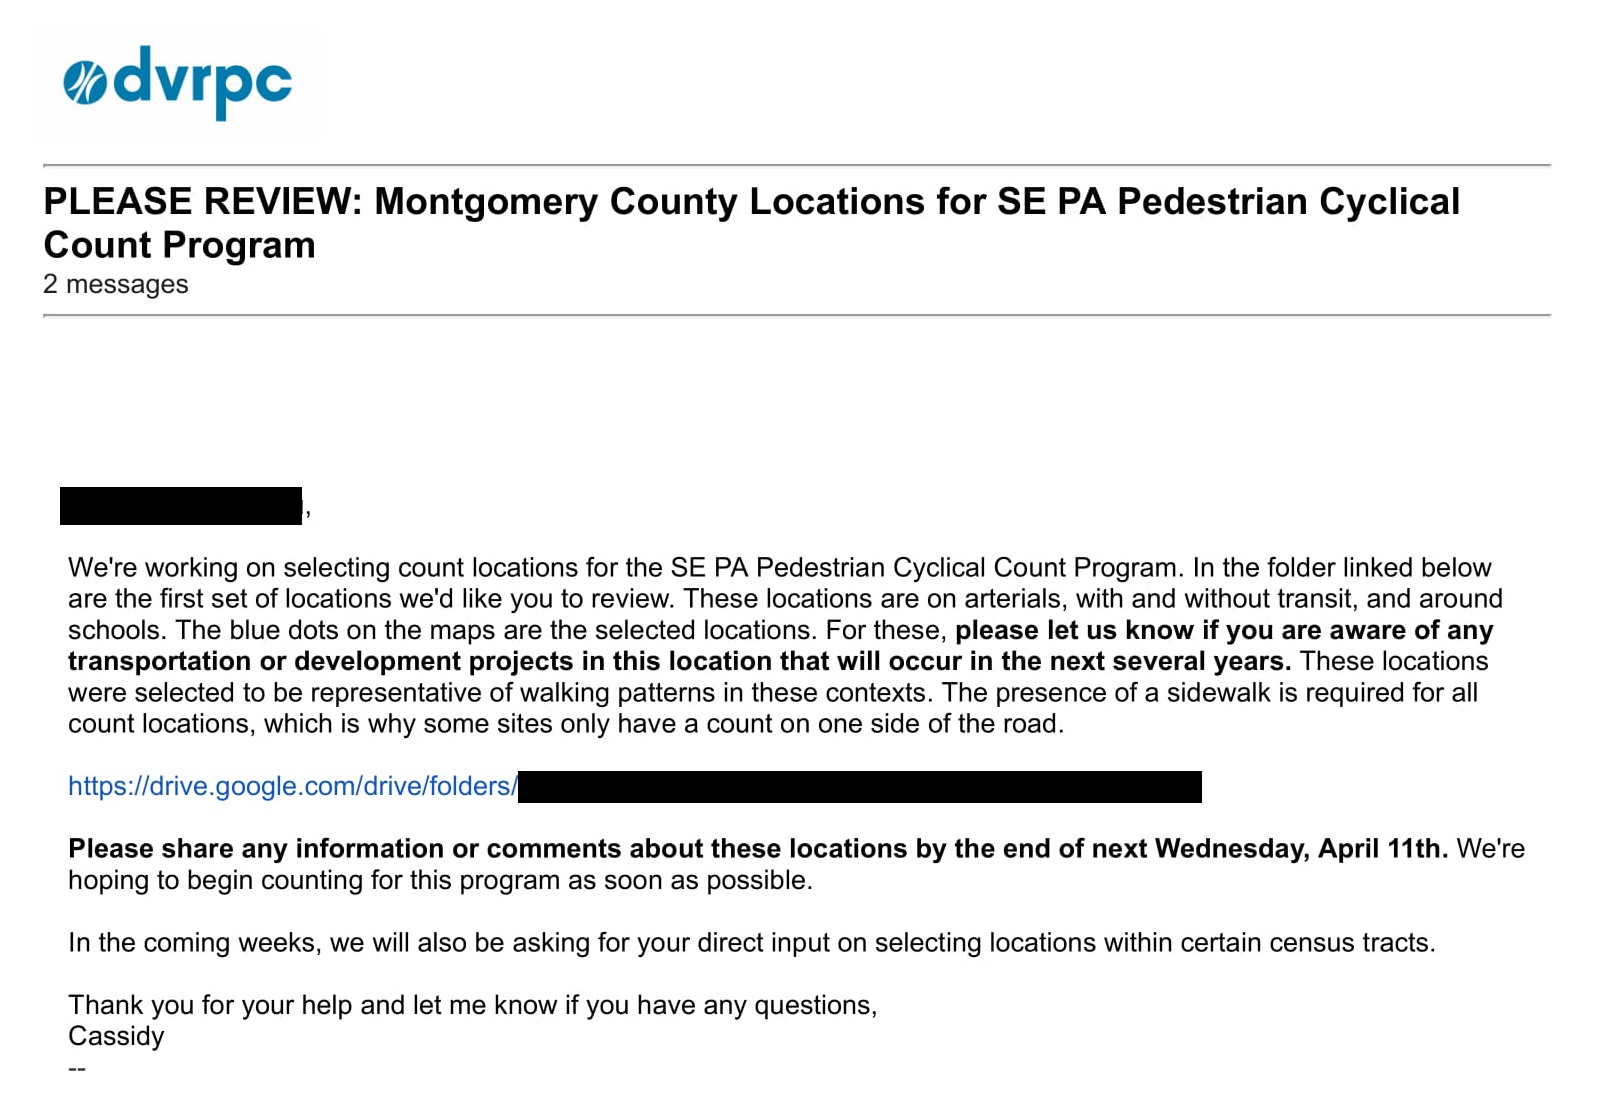
\includegraphics[width=\textwidth]{county-corresp-1.jpg}
	\caption{Correspondence with member governments regarding verification of arterial and school count locations.}
	\label{corresp-1}
\end{figure}
\FloatBarrier

\FloatBarrier
\begin{figure}[!htbp]
	\centering
	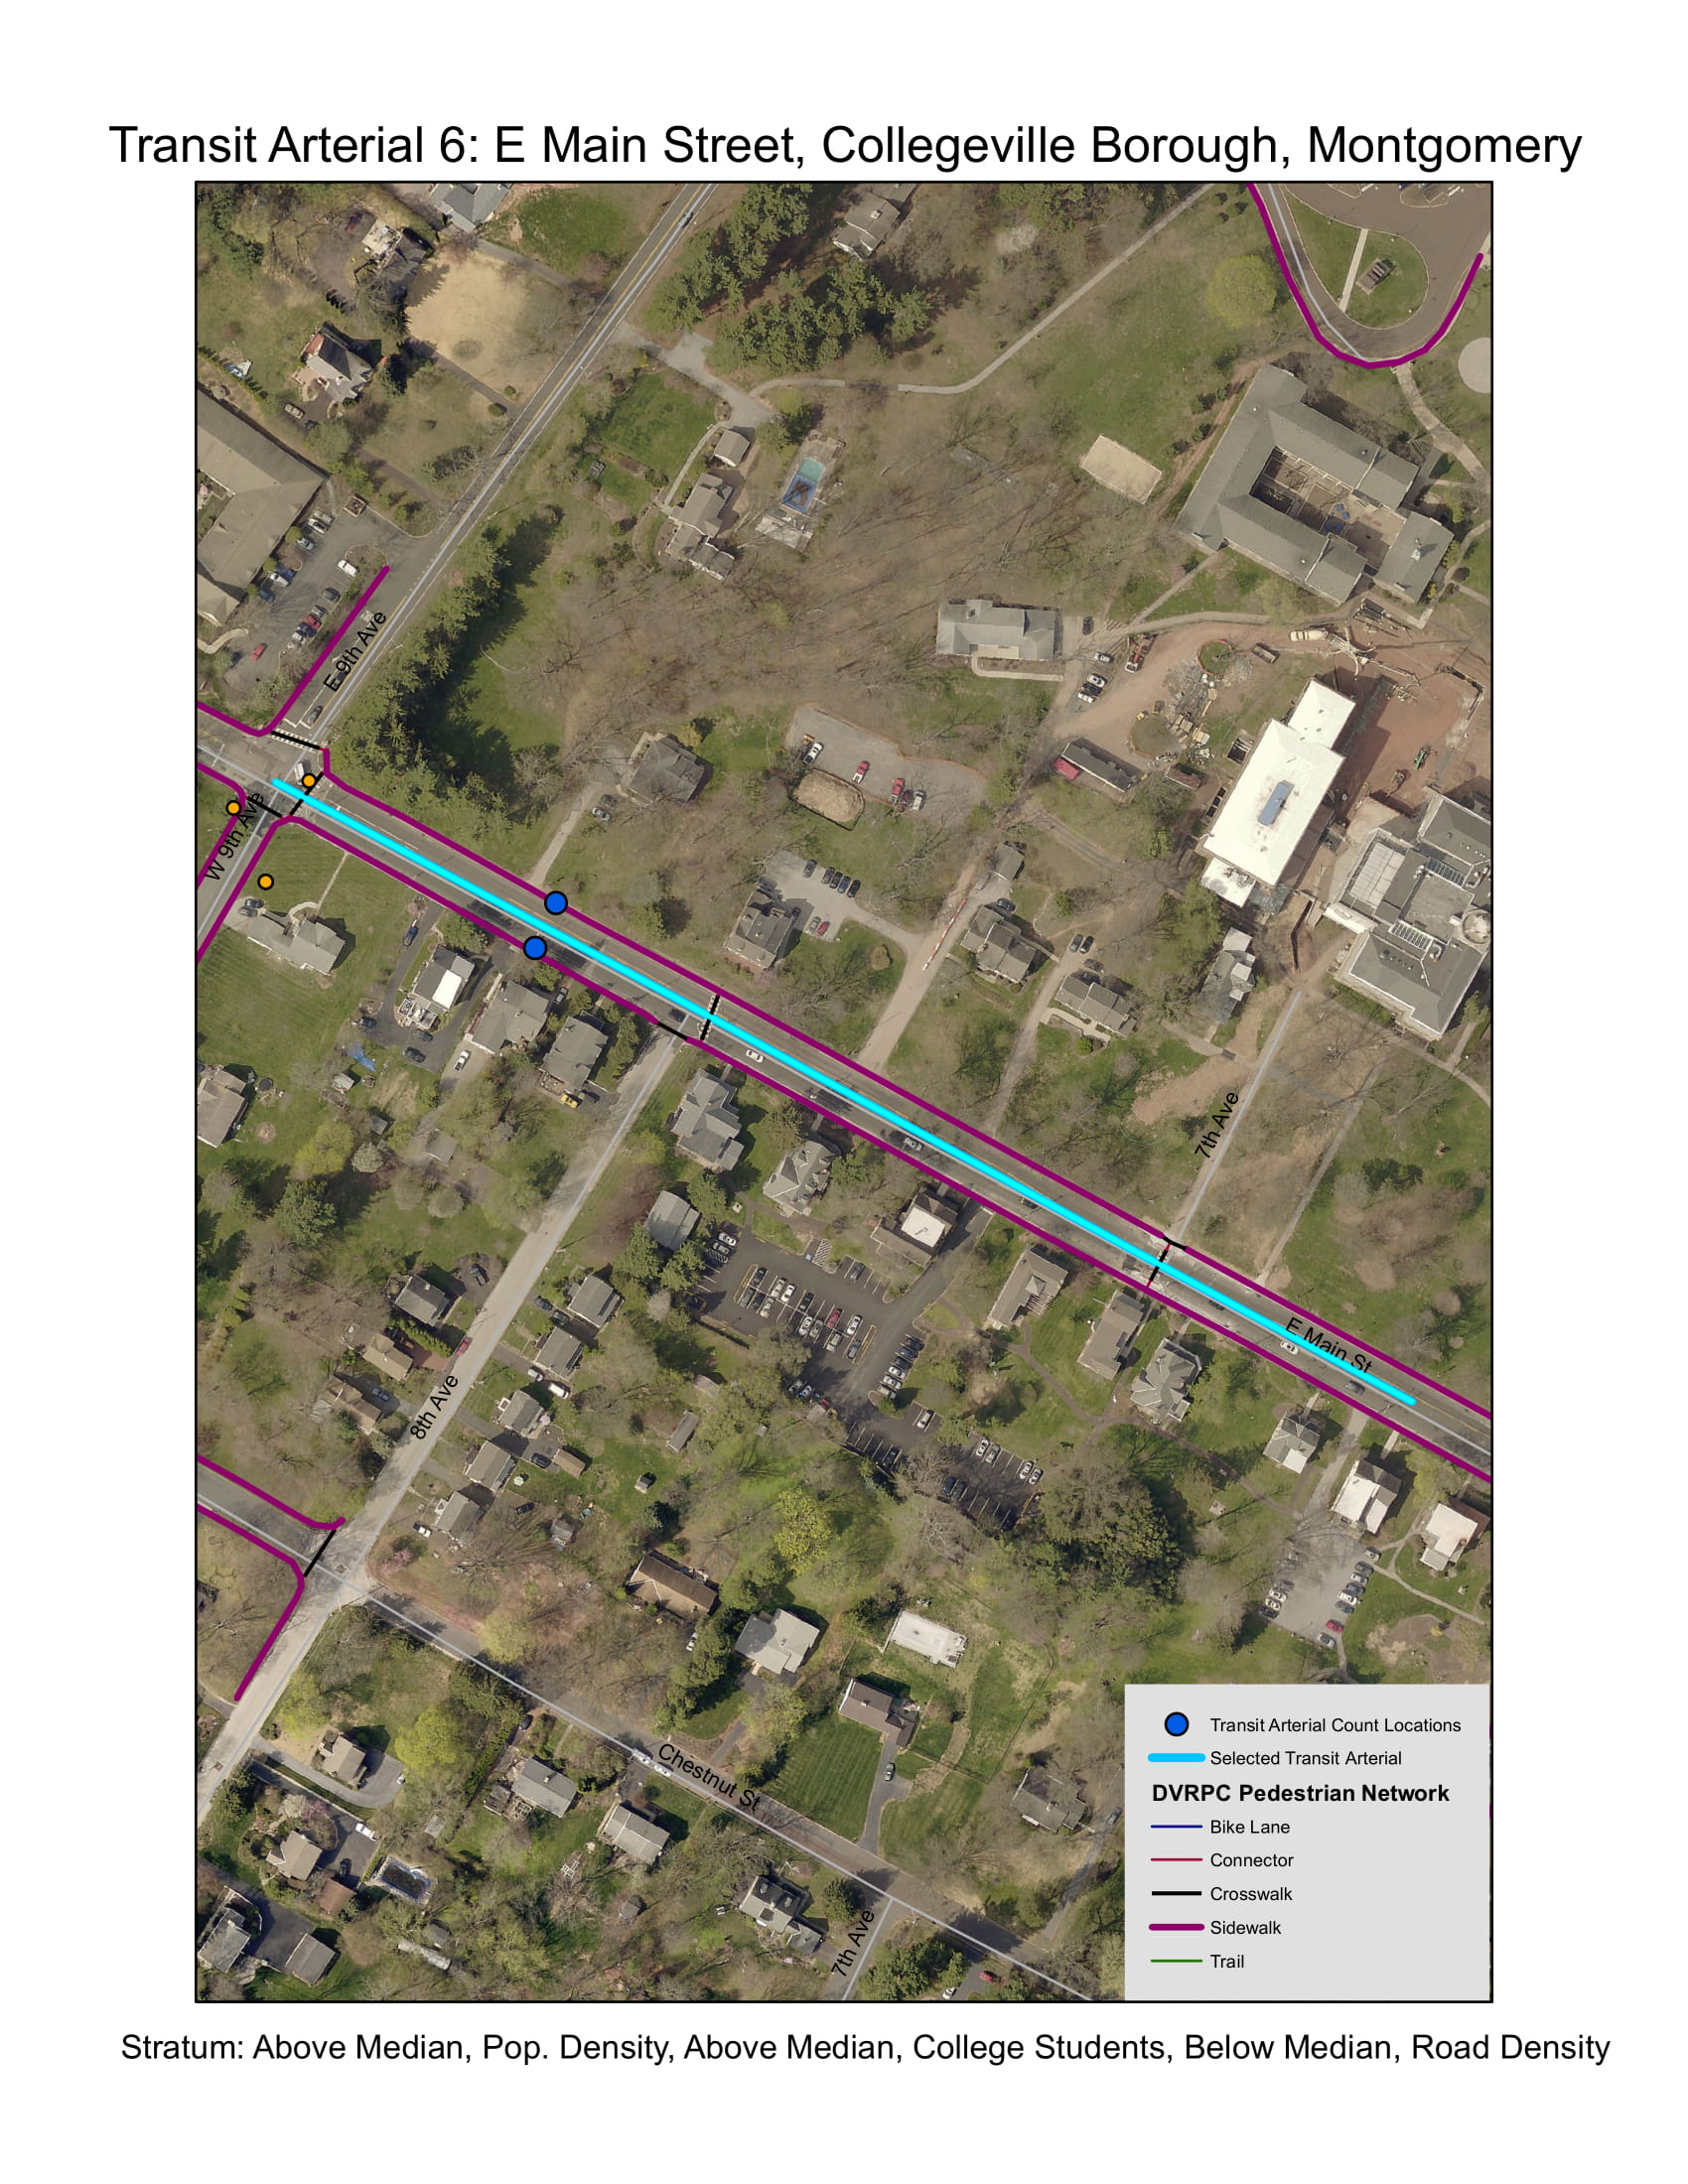
\includegraphics[width=\textwidth]{county-corresp-2.jpg}
	\caption{Sample transit arterial location sent to Montgomery County for review.}
	\label{corresp-2}
\end{figure}
\FloatBarrier

\FloatBarrier
\begin{figure}[!htbp]
	\centering
	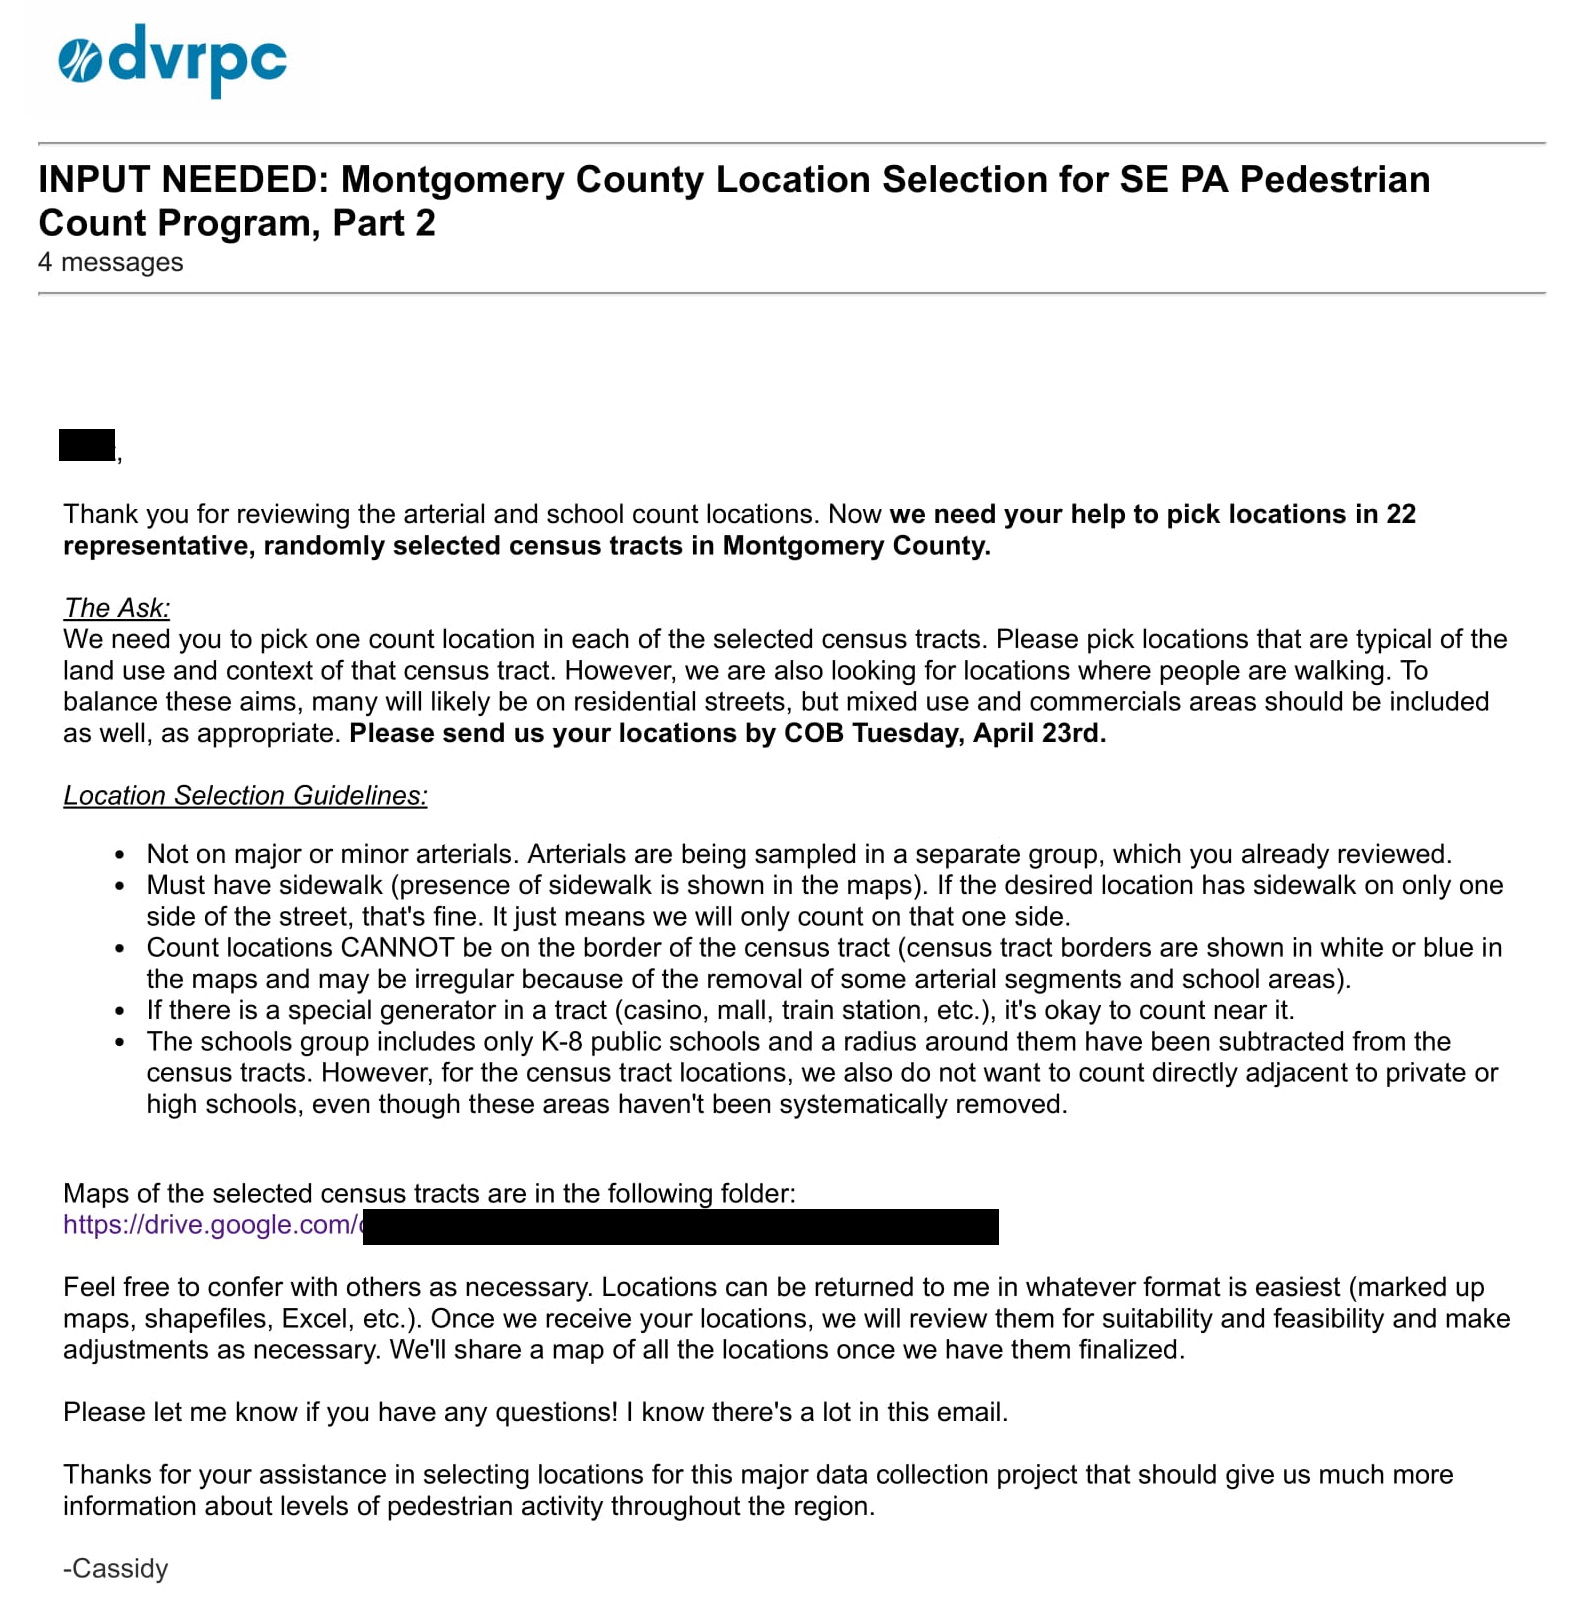
\includegraphics[width=\textwidth]{county-corresp-3.jpg}
	\caption{Correspondence with member governments regarding selection of census tract count locations.}
	\label{corresp-3}
\end{figure}
\FloatBarrier

\FloatBarrier
\begin{figure}[!htbp]
	\centering
	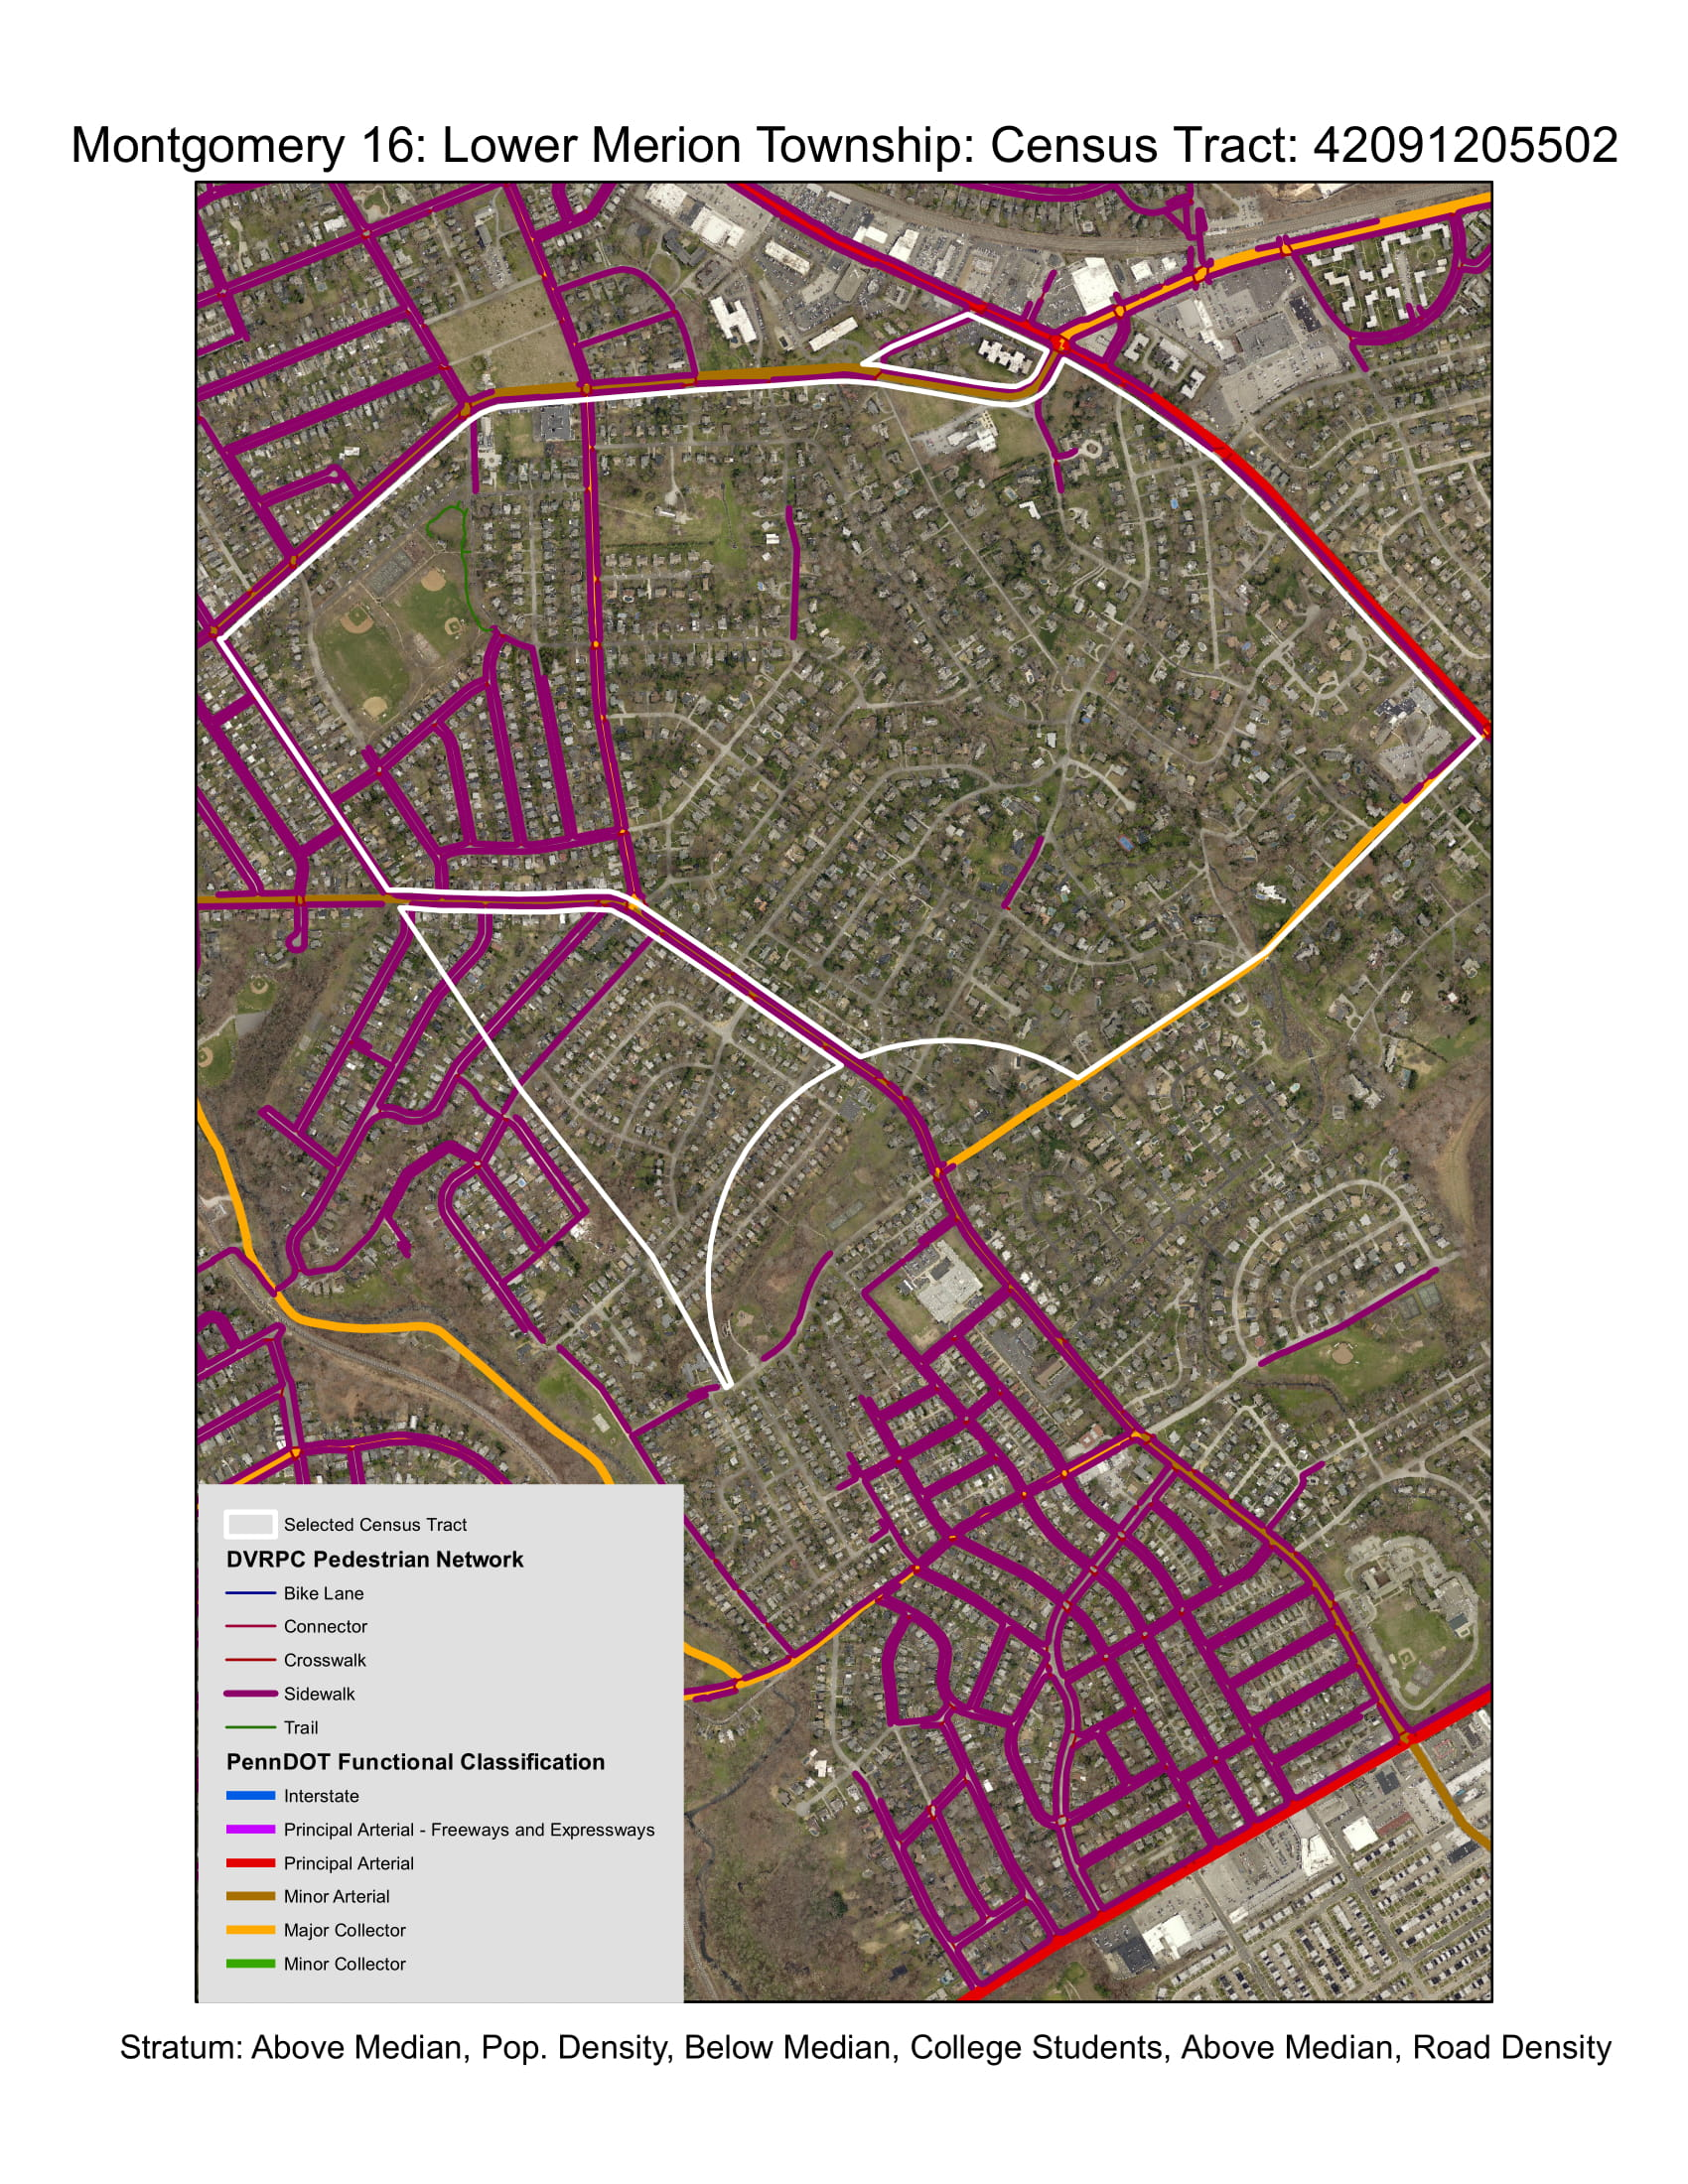
\includegraphics[width=\textwidth]{county-corresp-4.jpg}
	\caption{Sample census tract sent to Montgomery County to select a count location.}
	\label{corresp-4}
\end{figure}
\FloatBarrier

\section{In hindsight}
\label{sec:improvements}

The goal of the site selection process of DVRPC's SE Pennsylvania Cyclical Pedestrian Counting Program is to maximize the representativeness of on-street pedestrian count locations while minimizing bias. Our site selection process has accomplished this goal through stepwise regression and SRS, and counts are currently being conducted in the four suburban counties of the study area at the time of writing. We also minimize bias and maximize reproducibility by automating all steps of the site selection process in \texttt{R} except the verification of count locations. \\

In the future, we will be able to assess the representativeness of our site selection process using the counts collected from this program. For example, the sampling strata could be evaluated through a cluster analysis of all counts. If the sampling strata and the resulting clusters are similar, this may indicate that the sampling strata represent different pedestrian activity patterns. These results might then be used to extrapolate on-street pedestrian patterns to other locations where counts have not yet been conducted. \\

That said, there are opportunities for improvement in the design of this site selection process. While stratified random sampling of census tracts is good in that it allows member governments to become involved in the site selection process and the pedestrian count program more generally, it also increases the chances of biased site selection, as many census tracts have several eligible areas to conduct a pedestrian count. SRS of eligible road segments would reduce the potential for bias in site selection and enable us to consider road functional classification aside from major and minor arterials. \\

Our IDW interpolation method did not include any distance constraint. This means that the value assigned to a given grid cell of the 100,000 grid cells in the study area depended on the values of all on-street pedestrian counts in the region. It would be preferable to add a distance constraint so that the values of grid cells not within a reasonable distance of an existing count are not predicted. While this would reduce the number of census tracts to compare observed and estimated pedestrian densities, the results would likely be more realistic. \\

IDW interpolation is used in this study because it is easy to implement, and it would likely be difficult to fit a semivariogram to existing pedestrian counts given the paucity of available data. However, if a study area already has several existing counts, then kriging can be used to fit a model directly to existing counts. In their tests of ordinary and universal kriging versus IDW interpolation, Zimmerman et al. find that kriging performs better than IDW interpolation on irregular surfaces and when sample points are less uniformly distributed---both of which are expected attributes of non-motorized count data. A regression-kriging approach would combine regression with ordinary kriging and potentially enable the creation of sampling strata without needing to estimate pedestrians at the census tract level. \\

IDW interpolation and kriging incorporate the distance between observations in calculation; we use straight-line distances in this paper. It would be preferable to incorporate network distance into future approaches.


\bibliographystyle{apacite}
\bibliography{biblio}

\end{document}
